% SPDX-License-Identifier: CC-BY-SA-4.0
%
% Copyright (c) 2020 Philipp Le
%
% Except where otherwise noted, this work is licensed under a
% Creative Commons Attribution-ShareAlike 4.0 License.
%
% Please find the full copy of the licence at:
% https://creativecommons.org/licenses/by-sa/4.0/legalcode

\chapter{Spread Spectrum and Multiple Access}

\begin{refsection}
	
The electromagnetic spectrum is a sparse resource. It must be used as efficient as possible because it is shared with numerous users and applications. However, modern digital communication systems use spread spectrum technologies that occupy a relatively wide frequency band

The purpose of spread spectrum is amongst others:
\begin{itemize}
	\item Immunity against noise and disturbances
	\item Encryption and confidentiality of the communication
	\item Plausible deniability that the communication had ever taken place
	\item Coexistence with other services (multiple access)
\end{itemize}

Especially, the multiple access is an important reason for employing spread spectrum technologies. In modern communication systems, the resource \emph{frequency} is not only allocated to a single user. For example, \ac{LTE} allows many users to access the service with high data rates and low latency. The resource \emph{frequency} must be shared. Efficient medium access relies on spread spectrum to achieve this.

\section{Spread Spectrum}

In the modulation techniques considered so far, are \emph{plain} or \emph{non-spread spectrum}. For the definition of spread spectrum signals, the symbol duration and the transmission bandwidth is investigated.
\begin{itemize}
	\item The signal duration is the amount of time required to convey an information. In digital communication system, an information is a symbol modulated onto a carrier. The signal duration is the symbol period $T_{sym}$.
	\item The signal bandwidth $\Delta f_{sym}$ is the minimum bandwidth required by the receiver to receive the signal. In the case of modulation, it is the \emph{transmission bandwidth}.
\end{itemize}
In the \ac{ASK}, \ac{PSK} and \ac{QAM} modulation of Chapter 5, the signal duration and the bandwidth are inversely proportional.
\begin{equation}
	\Delta f_{sym} = \frac{1}{T_{sym}}
\end{equation}

The product of the bandwidth and the duration -- the \index{time-bandwidth product} \textbf{time-bandwidth product} -- is constantly $1$.\footnote{This is the ideal case. For real implementations, the constant may differ from $1$ depending on the modulation technique. However, it will be close to $1$.}
\begin{equation}
	T_{sym} \cdot \Delta f_{sym} = 1
\end{equation}

\paragraph{Time-Bandwidth Product.}

The time-bandwidth product is used for the definition of spread spectrum:
\begin{definition}{Spread spectrum}
	The time-bandwidth product of \index{spread spectrum} \textbf{spread spectrum} signals is significantly greater than $1$.
	\begin{equation}
		T_{sym} \cdot \Delta f_{sym} \gg 1
	\end{equation}
\end{definition}

Typically, this means that the bandwidth $\Delta f_{sym}$ is increased while the symbol duration and thereby the symbol rate is kept constant.
\begin{itemize}
	\item The symbol sequence (time-bandwidth product of $1$) is altered in a way which distributes the signal power over a wider frequency band. This process is called \index{spreading} \textbf{spreading}.
	\item The inverse process is \index{despreading} \textbf{despreading}. The original symbol sequence is reconstructed from the wide-band spread spectrum signal.
\end{itemize}

\begin{figure}[H]
	\centering
	\begin{tikzpicture}
		\begin{axis}[
			height={0.15\textheight},
			width=0.8\linewidth,
			scale only axis,
			xlabel={$\omega$},
			ylabel={$|\mathrm{S}_{XX}|$},
			%grid style={line width=.6pt, color=lightgray},
			%grid=both,
			grid=none,
			legend pos=north east,
			axis y line=middle,
			axis x line=middle,
			every axis x label/.style={
				at={(ticklabel* cs:1.05)},
				anchor=north,
			},
			every axis y label/.style={
				at={(ticklabel* cs:1.05)},
				anchor=east,
			},
			xmin=0,
			xmax=10.5,
			ymin=0,
			ymax=1.2,
			xtick={0},
			xticklabels={0},
			ytick={0},
			axis x discontinuity=parallel,
		]
			\addplot[blue, smooth] coordinates {(4.6,0) (4.7,0.02) (4.8,0.2) (4.9,0.71) (5,1) (5.1,0.71) (5.2,0.2) (5.3,0.02) (5.4,0)};
			\addlegendentry{Narrow-band signal};
			\addplot[red, smooth] coordinates {(2,0) (2.5,0.01) (3,0.05) (5,0.05) (7,0.05) (7.5,0.01) (8,0)};
			\addlegendentry{Spread spectrum signal};
		\end{axis}
	\end{tikzpicture}
	\caption[PSD of a narrow-band and spread spectrum signal]{\acs{PSD} of a narrow-band and spread spectrum signal. Both signals carry the same information and have the equal power. The narrow-band signal concentrates the whole signal power in a narrow frequency band. In contrast, the spread spectrum signal distributes the signal power over a wide frequency band.}
\end{figure}

\paragraph{Noise-like Signal.}

The signal power remains constant while the signal is spread.
\begin{itemize}
	\item The \ac{PSD} is reduced.
	\item But, the \ac{PSD} is integrated over a wider frequency range.
	\item The overall power remains constant.
\end{itemize}

The \ac{PSD} of the spread spectrum signal is flat in approximation.
\begin{itemize}
	\item The flat \ac{PSD} resembles the \ac{PSD} of noise.
	\item Spread spectrum signal are therefore \emph{noise-like}.
\end{itemize}

A third party who has no knowledge of neither the existence of the spread spectrum signal nor the technology used cannot detect the signal.
\begin{itemize}
	\item The spread spectrum signal looks like noise or a wide-band disturbance from the view of the receiver which does not participate in the communication.
	\item This circumstance can be used to conceal the existence of the signal (plausible deniability of its existence).
\end{itemize}

\paragraph{Despreading.}

\index{despreading} Despreading reconstructs the symbols -- and thereby the data -- from the spread spectrum signal.
\begin{itemize}
	\item The spreading is reversed.
	\item The symbols (time-bandwidth product of $1$) are reconstructed. This can be seen like re-concentrating the spread signal power in a narrow-band symbol sequence.
	\item The disturbances which are uncorrelated to the spread spectrum signal are converted into the wide-band noise with a low \ac{PSD}.
	\begin{itemize}
		\item The wide-band noise floor (like thermal noise or quantization noise) remains wide-band.
		\item Strong but narrow-band disturbing signals (like other users of the electromagnetic spectrum) are spread to low-\acs{PSD} wide-band noise during the despreading. The \ac{SNR} is increased by spreading the signal power of the disturbance.
	\end{itemize}
\end{itemize}

\subsection{Direct-Sequence Spread Spectrum}

A simple method for increasing the bandwidth systematically re-encoding the symbols using new symbols at a higher symbol rate.
\begin{itemize}
	\item The input symbols are at the rate of $f_{sym}$.
	\item The \emph{spreading} is achieved by re-encoding each symbol by $L$ new symbols, called \index{chip} \textbf{chips}.
	\item After re-encoding, the rate of the new symbols -- the \emph{chips} -- is $f_{chp}$. $f_{chp}$ is the \index{chip rate} \textbf{chip rate}. \nomenclature[Sf]{$f_{chp}$}{Chip rate}
	\item $L$ is the \index{spreading factor} \textbf{spreading factor}.
	\begin{equation}
		L = \frac{f_{chp}}{f_{sym}}
	\end{equation}
\end{itemize}

\begin{example}{\acs{IEEE} 802.11b (Wi-Fi)}
	\acs{IEEE} 802.11b is an early \ac{WLAN} standard from 1999, defining data rates of \SI{1}{Mbit/s} to \SI{11}{Mbit/s}.\footnote{In comparison to that, modern \ac{WLAN} standards like \acs{IEEE} 802.11ax have data rates of several \si{Gbit/s}. But they use other spread spectrum technologies.} Usually, the data rate is proportional to the transmission bandwidth. But, \acs{IEEE} 802.11b uses \ac{DSSS} to implement an adaptive data rate whilst retaining a constant bandwidth (approximately \SI{22}{MHz}).
	
	\begin{figure}[H]
		\centering
		\begin{circuitikz}
			\node[mixer](Spreader){};
			\node[draw,block,below=1.5cm of Spreader](Code){Code\\ generator};
			\node[draw,block,right=3cm of Spreader](Mod){\acs{BPSK}\\ modulator};
			
			\node[above=3mm of Spreader,align=center]{Multiplier as\\ the spreader};
			
			\draw[-o] (Spreader.west) node[inputarrow]{} -- ++(-1cm,0) node[left,align=right]{Input data\\ at $f_{sym}$};
			\draw (Code.north) -- node[midway,right,align=left]{Spreading code\\ at $f_{chip}$} (Spreader.south) node[inputarrow,rotate=90]{};
			\draw (Spreader.east) -- node[midway,above,align=center]{Chip\\ sequence} (Mod.west) node[inputarrow]{};
			\draw (Mod.east) -- ++(1cm,0) node[inputarrow]{} node[right,align=left]{Baseband\\ signal};
		\end{circuitikz}
		\caption{Simplified spreading and \acs{PSK} modulation signal chain of an \acs{IEEE} 802.11b conforming transmitter}
	\end{figure}

	Data is represented by bits. At a data rate of $f_{sym} = \SI{1}{Mbit/s}$, the data is spread by a factor $L = 11$. The data symbols are multiplied by the \emph{spreading code}. Because of the multiplication, the same block symbol as the mixer is used. The code has a \emph{chip rate} of $f_{chp} = L f_{sym} = \SI{11}{Mchp/s}$.\footnote{Physically, the units \si{bit} and \si{chp} are dimension-less. Therefore, $\SI{1}{Mbit/s} = \SI{1}{Mchp/s} = \SI{1}{MHz}$. However, the units shall refer to the quantity being considered.}
	
	\vspace{0.5em}
	
	For $L = 11$, the \index{Barker code} \textbf{Barker code} with $\vect{C}_{11} = \left[+1, +1, +1, -1, -1, -1, +1, -1, -1, +1, -1\right]$ is used as the spreading code. Let's consider a bit stream of $(10)_2$ as th data, which is encoded as the symbols $\vect{D} = \left[-1, +1\right]$. The spread sequence is:
	\begin{equation}
		\begin{split}
			\vect{S} &= \vect{D} \otimes \vect{C}_{11} \\
			 &= \left[\underbrace{-1, -1, -1, +1, +1, +1, -1, +1, +1, -1, +1}_{\text{Spread symbol } -1},\right. \\ &\qquad \left.  \underbrace{+1, +1, +1, -1, -1, -1, +1, -1, -1, +1, -1}_{\text{Spread symbol } +1}\right]
		\end{split}
	\end{equation}
	
	The \emph{chip sequence} $\vect{S}$ is at a rate of \SI{11}{Mchp/s}. In this case, the \emph{chip} have two discrete states $-1$ or $+1$. They can be modulated by a \ac{BPSK} modulator. It baseband is then mixed to the \ac{RF} band of \SI{2.4}{GHz} using an IQ modulator.
	
	\begin{figure}[H]
		\centering
		
		\subfloat[Data symbols]{
			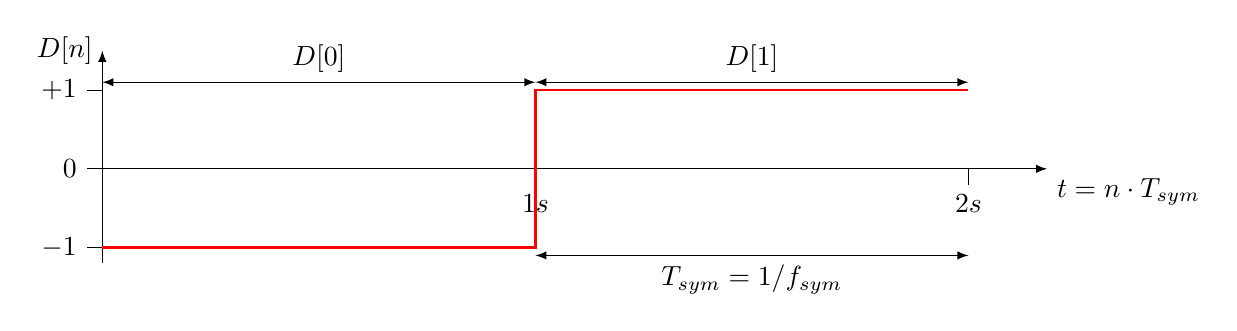
\begin{tikzpicture}
				\draw[-latex] (0,0) -- (12,0) node[below right, align=left]{$t = n \cdot T_{sym}$};
				\draw[-latex] (0,-1.2) -- (0,1.5) node[left, align=right]{$D[n]$};
				\foreach \y in {-1, 0, +1}{
					\draw (0,\y) -- (-0.2,\y) node[left,align=right]{$\y$};
				}
				\foreach \x/\t in {5.5/1, 11/2}{
					\draw (\x,0) -- (\x,-0.2) node[below,align=center]{$\SI{\t}{\micro{}s}$};
				}
			
				\foreach \x/\n in {0/0, 5.5/1}{
					\draw[latex-latex] (\x,1.1) -- node[midway,above,align=center]{$D[\n]$} ({\x+5.5},1.1);
				}
				
				\draw[red,thick] (0,-1) -- (5.5,-1) -- (5.5,1) -- (11,1);
				
				\draw[latex-latex] (5.5,-1.1) -- node[midway,below,align=center]{$T_{sym} = 1/f_{sym}$} (11,-1.1);
			\end{tikzpicture}
		}
	
		\subfloat[Code chips]{
			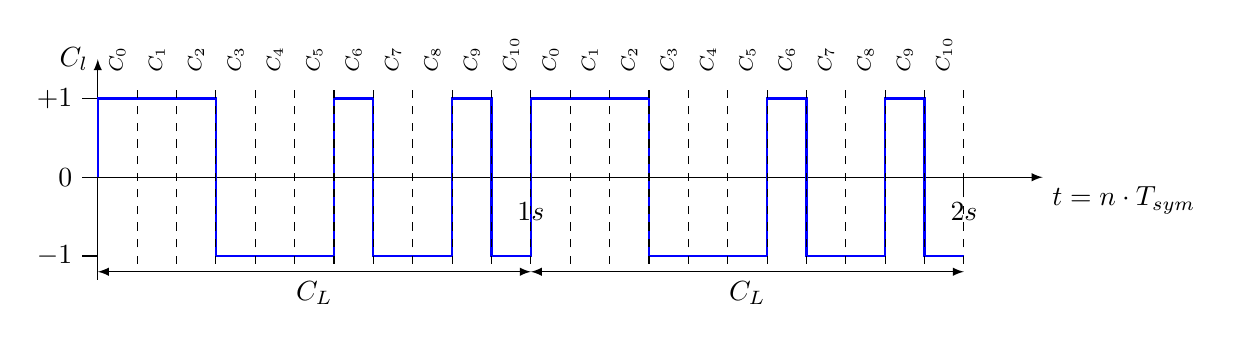
\begin{tikzpicture}
				\draw[-latex] (0,0) -- (12,0) node[below right, align=left]{$t = n \cdot T_{sym}$};
				\draw[-latex] (0,-1.3) -- (0,1.5) node[left, align=right]{$C_l$};
				\foreach \y in {-1, 0, +1}{
					\draw (0,\y) -- (-0.2,\y) node[left,align=right]{$\y$};
				}
				\foreach \x/\t in {5.5/1, 11/2}{
					\draw (\x,0) -- (\x,-0.2) node[below,align=center]{$\SI{\t}{\micro{}s}$};
				}
				
				\draw[blue,thick] (0,0) \foreach \n in {0, 1} {
					\foreach \l/\c in {0/+1, 1/+1, 2/+1, 3/-1, 4/-1, 5/-1, 6/+1, 7/-1, 8/-1, 9/+1, 10/-1}{
						-- ({(\n*5.5)+(\l*0.5)},\c) -- ({(\n*5.5)+(\l*0.5+0.5)},\c)
					}
				};
			
				%\draw[dashed] (5.5,-1.2) -- (5.5,1.2);
				%\draw[dashed] (11,-1.2) -- (11,1.2);
				\foreach \n in {0, 1} {
					\foreach \l in {0,1,...,10}{
						\node[anchor=west,rotate=90,align=center] at({((\n*11+\l)*0.5)+0.25},1.2) {\scriptsize $C_{\l}$};
						\draw[dashed] ({((\n*11+\l)+1)*0.5},-1.1) -- ({((\n*11+\l)+1)*0.5},1.2);
					}
				}
			
				\foreach \x/\n in {0/0, 5.5/1}{
					\draw[latex-latex] (\x,-1.2) -- node[midway,below,align=center]{$\vect{C}_L$} ({\x+5.5},-1.2);
				}
			\end{tikzpicture}
		}
	
		\subfloat[Output chips]{
			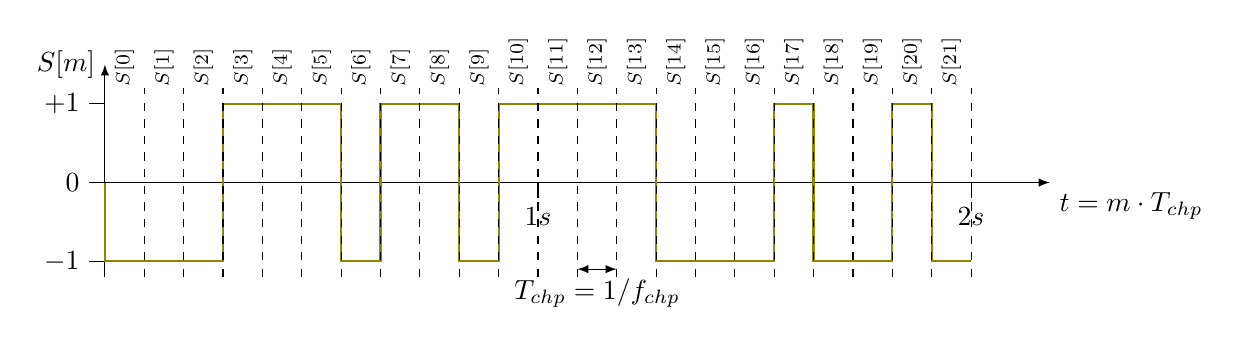
\begin{tikzpicture}
				\draw[-latex] (0,0) -- (12,0) node[below right, align=left]{$t = m \cdot T_{chp}$};
				\draw[-latex] (0,-1.2) -- (0,1.5) node[left, align=right]{$S[m]$};
				\foreach \y in {-1, 0, +1}{
					\draw (0,\y) -- (-0.2,\y) node[left,align=right]{$\y$};
				}
				\foreach \x/\t in {5.5/1, 11/2}{
					\draw (\x,0) -- (\x,-0.2) node[below,align=center]{$\SI{\t}{\micro{}s}$};
				}
				
				\draw[olive,thick] (0,0) \foreach \n/\d in {0/-1, 1/+1} {
					\foreach \l/\c in {0/+1, 1/+1, 2/+1, 3/-1, 4/-1, 5/-1, 6/+1, 7/-1, 8/-1, 9/+1, 10/-1}{
						-- ({(\n*5.5)+(\l*0.5)},{\c*\d}) -- ({(\n*5.5)+(\l*0.5+0.5)},{\c*\d})
					}
				};
			
				%\draw[dashed] (5.5,-1.2) -- (5.5,1.2);
				%\draw[dashed] (11,-1.2) -- (11,1.2);
				\foreach \m in {0,1,...,21}{
					\node[anchor=west,rotate=90,align=center] at({(\m*0.5)+0.25},1.1) {\scriptsize $S[\m]$};
					\draw[dashed] ({(\m+1)*0.5},-1.2) -- ({(\m+1)*0.5},1.2);
				}
			
				\draw[latex-latex] (6,-1.1) -- node[midway,below,align=center]{$T_{chp} = 1/f_{chp}$} (6.5,-1.1);
			\end{tikzpicture}
		}
	
		\caption{Data, spreading code and output chips of IEEE 802.11b symbols at a spreading factor of $L = 11$}
		\label{fig:ch07:wlan_dsss}
	\end{figure}
	
	At a data rate of \SI{11}{Mbit/s}, the data is \underline{not} spread ($L = 1$). The spreading code is $\vect{C}_{1} = \left[+1\right]$. The \emph{chip rate} equals the data bit rate. The \emph{chip rate} remains constant at \SI{11}{Mchp/s}.
	
	\vspace{0.5em}
	
	\textbf{Why adaptive data rate?} Spreading by $L = 11$ increases the \ac{SNR}. Each symbol is effectively repeated 11 times. This circumstance can be used to achieve a processing gain and increase noise immunity. The higher data rate at a lower spreading factor of $L = 1$ comes at the drawback of decreased noise immunity.
\end{example}

The \index{direct-sequence spread spectrum} \textbf{\acf{DSSS}} spreads the symbols by multiplying each data symbol with the whole spreading code.
\begin{itemize}
	\item The data symbol sequence is represented by the vector $\vect{D}$. A single data symbol is $D[n]$. \nomenclature[Sd]{$\vect{D}$}{Data symbol sequence}
	\begin{equation}
		\vect{D} = \left[D[0], D[1], \dots\right]
	\end{equation}
	\item The data comes at the rate of $f_{sym}$.
	\item The code sequence is represented by the $L$-dimensional vector $\vect{C}_L$. $L$ is the length of the code. A single chip of the code is $C_l$. \nomenclature[Sd]{$\vect{C}_L$}{Spreading code for direct-sequence spread spectrum}
	\begin{equation}
		\vect{C} = \left[C_0, C_1, \dots, C_{L-1}\right]
	\end{equation}
	\item The code repeats at $f_{sym}$. The rate of the single code chips is $f_{chp} = L f_{sym}$.
\end{itemize}
The process of multiplying each data symbol $D_n$ with the whole code sequence $\left[C_0, C_1, \dots, C_{L-1}\right]$ is represented by the \index{Kronecker product} \textbf{Kronecker product} $\otimes$. \nomenclature[Fk]{$\otimes$}{Kronecker product}
\begin{equation}
	\begin{split}
		\vect{S} &= \vect{D} \otimes \vect{C}_{L} \\
		S[m] &= S[n L + l] = D[n] \cdot C_l \qquad \forall 0 \leq l < L
	\end{split}
\end{equation}
$\vect{S} = \left[S[0], S[1], \cdots\right]$ is the sequence of output chips -- the \emph{spread spectrum signal}. The chips in $\vect{S}$ are at the chip rate of $f_{chp} = M f_{sym}$. \nomenclature[Ss]{$\vect{S}$}{Chip sequence of a spread spectrum signal}

\begin{figure}[H]
	\centering
	\begin{circuitikz}
		\node[draw,block](Spreader){Spreader\\ $\vect{D} \otimes \vect{C}_{L}$};
		\node[draw,block,below=1.5cm of Spreader](Code){Code\\ generator};
		\node[draw,block,right=2.5cm of Spreader](Mod){Modulation\\ (\acs{BPSK}, \acs{QPSK},\\ \acs{QAM}, ...)};
		
		\draw[-o] (Spreader.west) node[inputarrow]{} -- ++(-1cm,0) node[left,align=right]{Input symbol\\ sequence $\vect{D}$};
		\draw (Code.north) -- node[midway,right,align=left]{Spreading\\ code $\vect{C}_{L}$} (Spreader.south) node[inputarrow,rotate=90]{};
		\draw (Spreader.east) -- node[midway,above,align=center]{Chip\\ sequence\\ $\vect{S}$} (Mod.west) node[inputarrow]{};
		\draw (Mod.east) -- ++(1cm,0) node[inputarrow]{} node[right,align=left]{Baseband\\ signal};
	\end{circuitikz}
	\caption{Abstract \acs{DSSS}}
	\label{fig:ch07:abstract_dsss}
\end{figure}

Figure \ref{fig:ch07:abstract_dsss} depicts an abstract view on \ac{DSSS}. The \emph{spreading code} is a \index{pseudorandom code} \textbf{pseudorandom code}.
\begin{itemize}
	\item The code is generated by an algorithm and is thereby predictable if the algorithm is known.
	\item For a receiver that does not know the code generation algorithm, the code sequence is random. It is noise-like.
	\item \textit{The fact, that the code must be known to the receiver, can be used to implement data \texttt{}encryption.}
\end{itemize}

Time-bandwidth product:
\begin{itemize}
	\item The bandwidth of the signal is the \emph{chip rate} $f_{chp}$. It is $L$ times the bandwidth of a non-spread symbol.
	\item The symbol period is not touched and remains $T_{sym}$.
	\item The transmission bandwidth of a non-spread symbol $\frac{1}{T_{sym}}$.
	\item The time-bandwidth product is
	\begin{equation}
		T_{sym} \cdot \Delta f_{chp} = T_{sym} \cdot \frac{L}{T_{sym}} = L \gg 1
	\end{equation}
	\item The \ac{DSSS} fulfils the spread spectrum condition.
\end{itemize}

Example usage of \ac{DSSS}:
\begin{itemize}
	\item \acs{IEEE} 802.11b specification for \ac{WLAN}
	\item \ac{GPS}
\end{itemize}

\subsection{Frequency-Hopping Spread Spectrum}

Another straightforward method spreading a signal across the frequency spectrum is transmitting each symbol at another frequency. This technique is called \index{frequency-hopping spread spectrum} \textbf{\acf{FHSS}}.
\begin{itemize}
	\item The frequency band $\Delta f_{FHSS}$ is divided into $M$ \index{sub-band} \textbf{sub-bands} with a bandwidth of $\Delta f_{sub}$. \nomenclature[Sf]{$\Delta f_{sub}$}{Bandwidth of a sub-band}
	\begin{equation}
		\Delta f_{sub} = \frac{\Delta f_{FHSS}}{M}
		\label{eq:ch07:fhss_sub_f}
	\end{equation}
	\item The bandwidth of the sub-band $\Delta f_{sub}$ is the transmission bandwidth of a single, non-spread symbol. $\Delta f_{sub}$ is wide enough to accommodate a symbol.
	\item Each symbol is transmitted in a different sub-band $k$ ($0 \leq k < M$).
	\item The sub-band n is selected according to the certain pattern, which is again called \index{spreading code} \textbf{spreading code}.
\end{itemize}

\begin{figure}[H]
	\centering
	\begin{circuitikz}
		\node[draw,block](Mod){Modulation\\ (\acs{BPSK}, \acs{QPSK},\\ \acs{QAM}, ...)};
		\node[draw,block](Code) at([yshift=-3.5cm]Mod) {Code\\ generator};
		\node[mixer,right=2.5cm of Mod](Mix){};
		\node[oscillator](LO) at([yshift=-3.5cm,xshift=5mm]Mix) {};
		
		\node[right=3mm of LO,align=left]{\acs{LO}};
		
		\draw[-o] (Mod.west) node[inputarrow]{} -- ++(-1cm,0) node[left,align=right]{Input symbol\\ sequence $\vect{D}$};
		\draw (Mod.east) -- node[midway,above,align=center]{Baseband\\ signal} (Mix.west) node[inputarrow,rotate=0]{};
		\draw (Code.east) -- node[midway,below,align=center]{Spreading\\ code $C_M[n]$} (LO.west) node[inputarrow,rotate=0]{};
		\draw (LO.north) -- node[midway,right,align=left]{Carrier} (Mix.south) node[inputarrow,rotate=90]{};
		\draw (Mix.east) -- ++(1cm,0) node[inputarrow]{} node[right,align=left]{\acs{RF}\\ signal};
	\end{circuitikz}
	\caption{Simplified block diagram of a \acs{FHSS} transmitter}
\end{figure}

Following can be said about the \emph{spreading code}:
\begin{itemize}
	\item The values of the \emph{spreading code} $C_M[n]$ define the sub-band $k$ where the symbol $D_n$ shall be transmitted. \nomenclature[Sd]{$\vect{C}_;$}{Spreading code for time-hopping or frequency-hopping spread spectrum}
	\begin{equation}
		k = C_M[n] \qquad , 0 \leq C_M[n] < M
		\label{eq:ch07:fhss_sub_index}
	\end{equation}
	One code sample $C_M[n]$ corresponds to the data symbol $D[n]$.
	\item The length of the \emph{spreading code} is generally not restricted. It can be repeating. But a repeating pattern is not required.
	\item The rule which generates the \emph{spreading code} (the algorithm) must be known to both the transmitter and receiver.
\end{itemize}

If $f_c$ is the centre frequency of the carrier, the exact transmission frequency $f_{n}$ of the symbol $S_n$ is:
\begin{equation}
	\begin{split}
		f_n &= \underbrace{f_c - \frac{\Delta f_{FHSS}}{2} + \frac{\Delta f_{sub}}{2}}_{\text{Centre frequency of the 1st sub-band}} + \underbrace{k \cdot \Delta f_{sub}}_{\text{Sub-band centre frequency offset}} \\
		 &\quad \text{Using \eqref{eq:ch07:fhss_sub_f} and \eqref{eq:ch07:fhss_sub_index}:} \\
		 &= f_c - \frac{M \cdot \Delta f_{sub}}{2} + \frac{\Delta f_{sub}}{2} + C_M[n] \cdot \Delta f_{sub} \\
		 &= f_c + \Delta f_{sub} \left(\frac{1-M}{2} + C_M[n] \right)
	\end{split}
\end{equation}

\begin{example}{\acs{FHSS}}
	Let's consider an example symbol sequence $\vect{D}$ with a length of $6$. The signal is spread by $M =4$.
	
	The spreading code generated by the algorithm is:
	\begin{equation}
		\vect{C}_4[n] = \left[C_4[0], C_4[1], \dots\right] = \left[1,0,3,2,0,1,\dots\right]
	\end{equation}
	
	The frequency usage can be plotted over time:
	\begin{figure}[H]
		\centering
		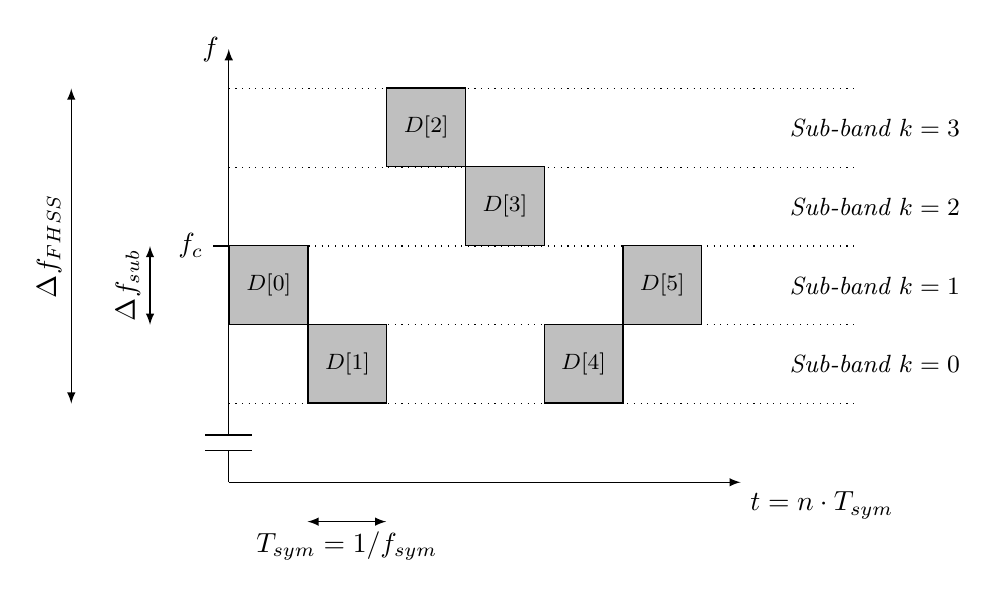
\begin{tikzpicture}[x=1cm,y=1cm]
			\draw[-latex] (0,0) -- (6.5,0) node[below right, align=left]{$t = n \cdot T_{sym}$};
			\draw[-latex] (0,0) -- (0,0.4) (0,0.6) -- (0,5.5) node[left, align=right]{$f$};
			\draw (-0.3,0.4) -- (0.3,0.4);
			\draw (-0.3,0.6) -- (0.3,0.6);
			
			\draw (0,3) -- (-0.2,3) node[left,align=right]{$f_c$};
			\draw[latex-latex] (-1,2) -- node[midway,left,align=center,anchor=south,rotate=90]{$\Delta f_{sub}$} (-1,3);
			\draw[latex-latex] (-2,1) -- node[midway,left,align=center,anchor=south,rotate=90]{$\Delta f_{FHSS}$} (-2,5);
			\draw[latex-latex] (1,-0.5) -- node[midway,below,align=center]{$T_{sym} = 1/f_{sym}$} (2,-0.5);
		
			\foreach \k in {0, 1, 2, 3}{
				\draw[dotted] (0,{\k+1}) -- (8,{\k+1});
				\node[right,align=left] at(7,{\k+1.5}) {\small\itshape Sub-band $k = \k$};
			}
			\draw[dotted] (0,5) -- (8,5);
			
			\foreach \n/\c in {0/1, 1/0, 2/3, 3/2, 4/0, 5/1}{
				\node[fill=gray!50, draw=black, minimum size=1cm, anchor=south west] at({\n},{\c+1}) {\footnotesize $D[\n]$};
			}
		\end{tikzpicture}
		\caption[Time-frequency plot of a symbol sequence spread by a \acs{FHSS} with $M = 4$]{Time-frequency plot of a symbol sequence spread by a \acs{FHSS} with $M = 4$. The $M = 4$ sub-bands are distributed around the centre frequency $f_c$. Each sub-band has the bandwidth $\Delta f_{sub}$. The duration of one symbol is $T_{sym}$ (symbol period).}
		\label{fig:ch07:fhss_ex}
	\end{figure}

	Each symbol in Figure \ref{fig:ch07:fhss_ex} is modulated (\ac{BPSK}, \ac{QPSK}, \ac{QAM}, ...).
\end{example}

Time-bandwidth product:
\begin{itemize}
	\item The bandwidth of the signal is $\Delta f_{FHSS} = M \Delta f_{sub}$. It is $M$ times the bandwidth of a non-spread symbol.
	\item The symbol period is not touched and remains $T_{sym}$.
	\item The sub-band bandwidth is the transmission bandwidth of a non-spread symbol $\Delta f_{sub} = \frac{1}{T_{sym}}$.
	\item The time-bandwidth product is
	\begin{equation}
		T_{sym} \cdot \Delta f_{FHSS} = M \gg 1
	\end{equation}
	\item The \ac{FHSS} fulfils the spread spectrum condition.
\end{itemize}

Benefits:
\begin{itemize}
	\item The benefits are the same as for \ac{DSSS} and other \emph{spread spectrum} techniques.
	\item The noise and disturbance immunity is improved.
\end{itemize}

Example usage of \ac{FHSS}:
\begin{itemize}
	\item \acs{IEEE} 802.15.1 (Bluetooth) -- Bluetooth employs a more sophisticated frequency-hopping scheme. The sub-bands are not spaced equally. The sub-band are located in the gaps between the \ac{WLAN} bands in the \SI{2.4}{GHz} band. This reduces the mutual interference of Bluetooth and \ac{WLAN}. Both services can coexists with minimum disturbance.
\end{itemize}

\subsection{Time-Hopping Spread Spectrum}

A third way of spreading the signal power across the frequency is shortening the symbol width $T_{chp}$ while keeping time symbol repetition period $T_{sym}$ constant. This technique is called \index{time-hopping spread spectrum} \textbf{\acf{THSS}}.
\begin{itemize}
	\item The transmission bandwidth is increased to $f_{sym} = \frac{1}{T_{chp}}$.
	\item The symbol is now a pulse -- called \index{chip} \textbf{chip} -- in the time-domain with a width of $T_{chp}$. A rest of the time portion, until the next symbol is transmitted, is zero.
	\item The pulse/symbol width is related to the symbol period $T_{sym}$.
	\begin{equation}
		T_{sym} = M \cdot T_{chp}
	\end{equation}
	\item The time-bandwidth product is
	\begin{equation}
		T_{sym} f_{sym} = M T_{chp} \frac{1}{T_{chp}} = M \gg 1
	\end{equation}
	The requirement for \emph{spread spectrum} signals is fulfilled.
\end{itemize}

The shortened pulse is then shifted in time.
\begin{itemize}
	\item The symbol period $T_{sym}$ is divided into $M$ time slots of equal length $T_{chp} = \frac{T_{sym}}{M}$.
	\item The shortened symbol is shifted to the $n$-th time slot.
	\item The values of the \emph{spreading code} $C_M[n]$ define the time slot $m$ (pulse position) where the pulse of the symbol $D_n$ shall be transmitted.
	\begin{equation}
		m = C_M[n] \qquad , 0 \leq C_M[n] < M
		\label{eq:ch07:thss_sub_index}
	\end{equation}
	One code sample $C_M[n]$ corresponds to the data symbol $D[n]$.
	\item The length of the \emph{spreading code} is generally not restricted. It can be repeating. But a repeating pattern is not required.
	\item The rule which generates the \emph{spreading code} (the algorithm) must be known to both the transmitter and receiver.
\end{itemize}

\begin{figure}[H]
	\centering
	\begin{circuitikz}
		\node[draw,block](Mod){Modulation\\ (\acs{BPSK}, \acs{QPSK},\\ \acs{QAM}, ...)};
		\node[draw,block,right=1.5cm of Mod](Shifter){Time-shifter\\ and pulse shaper};
		\node[draw,block,below=2cm of Shifter](Code){Code\\ generator};
		
		\draw[-o] (Mod.west) node[inputarrow]{} -- ++(-1cm,0) node[left,align=right]{Input symbol\\ sequence $\vect{D}$};
		\draw (Mod.east) -- (Shifter.west) node[inputarrow,rotate=0]{};
		\draw (Code.north) -- node[midway,right,align=left]{Spreading\\ code $C_M[n]$} (Shifter.south) node[inputarrow,rotate=90]{};
		\draw (Shifter.east) -- ++(1cm,0) node[inputarrow]{} node[right,align=left]{Baseband signal\\ (chip sequence $\vect{S}$)};
	\end{circuitikz}
	\caption[Simplified block diagram of a \acs{THSS} transmitter]{Simplified block diagram of a \acs{THSS} transmitter. The time-shifter and pulse shaper play a key role. The pulse shaper forms the shortened pulse with a width of $T_{chp} = \frac{T_{sym}}{M}$. The time-shifter shifts the pulse to the $C_n$-th time slot.}
\end{figure}

The output chip sequence $\vect{S} = \left[S[0], S[1], \dots\right]$ is at the rate $f_{chp} = M \cdot f_{sym}$. It is defined by:
\begin{equation}
	S[m] = S[n M + l] = \begin{cases}
		D[n] &\quad \text{if } l = C_M[n], \\
		0 &\quad \text{if } l \neq C_M[n].
	\end{cases}
\end{equation}

\begin{example}{\acs{THSS}}
	A data symbol sequence is spread by the spreading code:
	\begin{equation}
		\vect{C}_4[n] = \left[C_4[0], C_4[1], \dots\right] = \left[1,3,\dots\right]
	\end{equation}
	
	\begin{figure}[H]
		\centering
		
		\subfloat[Data symbols]{
			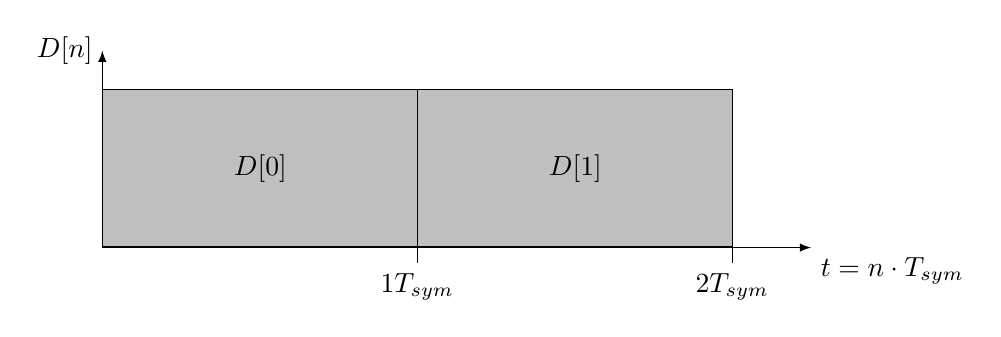
\begin{tikzpicture}[x=1cm,y=1cm]
				\draw[-latex] (0,0) -- (9,0) node[below right, align=left]{$t = n \cdot T_{sym}$};
				\draw[-latex] (0,0) -- (0,2.5) node[left, align=right]{$D[n]$};
				\foreach \x/\t in {4/1, 8/2}{
					\draw (\x,0) -- (\x,-0.2) node[below,align=center]{$\t T_{sym}$};
				}
			
				\foreach \n in {0, 1}{
					\node[fill=gray!50, draw=black, minimum width=4cm, minimum height=2cm, anchor=south west] at({\n*4},0) {$D[\n]$};
				}
			\end{tikzpicture}
		}
	
		\subfloat[Spreading code]{
			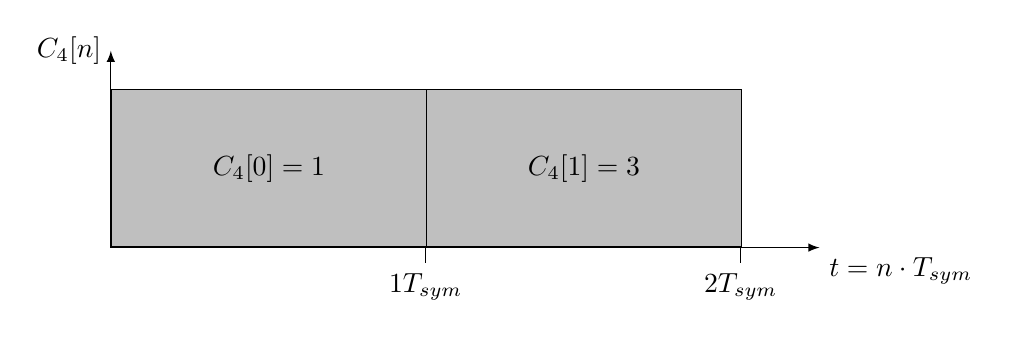
\begin{tikzpicture}
				\draw[-latex] (0,0) -- (9,0) node[below right, align=left]{$t = n \cdot T_{sym}$};
				\draw[-latex] (0,0) -- (0,2.5) node[left, align=right]{$C_4[n]$};
				\foreach \x/\t in {4/1, 8/2}{
					\draw (\x,0) -- (\x,-0.2) node[below,align=center]{$\t T_{sym}$};
				}
				
				\foreach \n/\c in {0/1, 1/3}{
					\node[fill=gray!50, draw=black, minimum width=4cm, minimum height=2cm, anchor=south west] at({\n*4},0) {$C_4[\n] = \c$};
				}
			\end{tikzpicture}
		}
		
		\subfloat[Output chips]{
			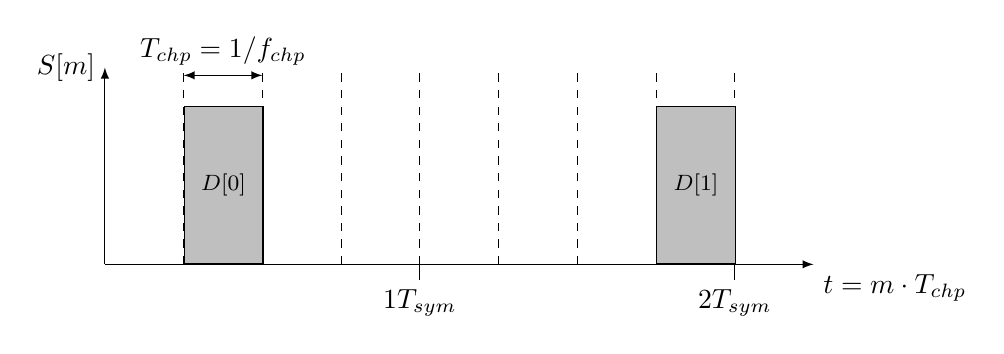
\begin{tikzpicture}
				\draw[-latex] (0,0) -- (9,0) node[below right, align=left]{$t = m \cdot T_{chp}$};
				\draw[-latex] (0,0) -- (0,2.5) node[left, align=right]{$S[m]$};
				\foreach \x/\t in {4/1, 8/2}{
					\draw (\x,0) -- (\x,-0.2) node[below,align=center]{$\t T_{sym}$};
				}
			
				\foreach \n in {0, 1}{
					\foreach \m in {1, 2, 3, 4}{
						\draw[dashed] ({(\n*4)+(\m)},0) -- ({(\n*4)+(\m)},2.5);
					}
				}
			
				\foreach \n/\c in {0/1, 1/3}{
					\node[fill=gray!50, draw=black, minimum width=1cm, minimum height=2cm, anchor=south west] at({(\n*4)+(\c)},0) {\footnotesize $D[\n]$};
				}
			
				\draw[latex-latex] (1,2.4) -- node[midway,above,align=center]{$T_{chp} = 1/f_{chp}$} (2,2.4);
			\end{tikzpicture}
		}
		
		\caption[\ac{THSS} signal]{\ac{THSS} signal. The symbol is shortened to a chip whose position is chosen by the spreading code.}
	\end{figure}
\end{example}

Benefits are the same as in other spread spectrum techniques. The noise immunity is improved.

Example usage of \ac{THSS}:
\begin{itemize}
	\item \ac{UWB} systems conforming to \acs{IEEE} 802.15.4
\end{itemize}

\subsection{Symbol Reconstruction}

\index{despreading} \textbf{Despreading} reconstructs the symbol sequence from the received \emph{spread spectrum} signal.

A despreader uses a cross-correlator to detect the spread symbols in the received signal. Remember that this is one of the purposes of cross-correlation.
\begin{itemize}
	\item The received signal is correlated with the \emph{spreading code}.
	\item The symbols spread with the same \emph{spreading code} can thereby be detected in the received signal.
\end{itemize}

\begin{remark}
	You may wonder why the autocorrelation is not used. Both receiver and transmitter use the same \emph{spreading code}. In deed, this a common misunderstanding. The received signal is different from the code and from the transmitted signal. The received signal contains noise and is subject to the transfer function of the transmission channel.
\end{remark}

\begin{figure}[H]
	\centering
	\begin{adjustbox}{scale=0.7}
		\begin{circuitikz}
			\node[draw,block](Demod){Demodulation\\ (\acs{BPSK}, \acs{QPSK},\\ \acs{QAM}, ...)};
			\node[draw,block,right=3cm of Demod](Corr){Cross corelation};
			\node[draw,block,below=1.5cm of Corr](Code){Code\\ generator};
			\node[draw,block,right=1.5cm of Corr](Det){Detector};
			
			\draw[-o] (Demod.west) node[inputarrow]{} -- ++(-1cm,0) node[left,align=right]{Received signal $r(t)$};
			\draw (Code.north) -- node[midway,right,align=left]{Spreading\\ code $\vect{C}$} (Corr.south) node[inputarrow,rotate=90]{};
			\draw (Demod.east) -- node[midway,above,align=center]{Received chip\\ sequence $\vect{R}$} (Corr.west) node[inputarrow]{};
			\draw (Corr.east) -- node[midway,above,align=center]{$\mathrm{R}_{RC}$} (Det.west) node[inputarrow]{};
			\draw (Det.east) -- ++(1cm,0) node[inputarrow]{} node[right,align=left]{Data};
		\end{circuitikz}
	\end{adjustbox}
	\caption{Abstract despreader using a cross-correlator}
	\label{fig:ch07:abstract_spreader}
\end{figure}

\subsubsection{Despreading of DSSS Signals}

\begin{figure}[H]
	\centering
	\begin{adjustbox}{scale=0.7}
		\begin{circuitikz}
			\node[draw,block](Demod){Demodulation\\ (\acs{BPSK}, \acs{QPSK},\\ \acs{QAM}, ...)};
			\node[mixer,right=3cm of Demod](Mul){};
			\node[draw,block,right=1cm of Mul](Acc){Accumulator};
			\node[draw,block,below=2cm of Mul](Code){Code\\ generator};
			\node[draw,block,right=1cm of Acc](Det){Detector};
			
			\node[above=3mm of Mul,align=center]{Multiplier as\\ despreader};
			
			\draw[-o] (Demod.west) node[inputarrow]{} -- ++(-1cm,0) node[left,align=right]{Received signal $r(t)$};
			\draw (Code.north) -- node[midway,right,align=left]{Spreading\\ code $\vect{C}_L$} (Mul.south) node[inputarrow,rotate=90]{};
			\draw (Demod.east) -- node[midway,below,align=center]{Received chips\\ $\vect{R}$} (Mul.west) node[inputarrow]{};
			\draw (Mul.east) -- (Acc.west) node[inputarrow]{};
			\draw (Acc.east) -- (Det.west) node[inputarrow]{};
			\draw (Det.east) -- ++(1cm,0) node[inputarrow]{} node[right,align=left]{Data};
			
			\draw[dashed] ([shift={(5mm,2cm)}]Acc.north east) node[anchor=south east,align=right]{Cross-correlation} -- ++(0,-3.5cm) -- ++(-7cm,0) -- ++(0,3.5cm) -- cycle;
		\end{circuitikz}
	\end{adjustbox}
	\caption{Simplified \acs{DSSS} despreader}
	\label{fig:ch07:abstract_dsss_spreader}
\end{figure}

\begin{itemize}
	\item The spreading, which was a multiplication of the data with the \emph{spreading code}, is reversed by multiplying the received chips again with the \emph{spreading code}.
	\item The accumulation then sums up the correlated chips.
	\item When the full code length has been accumulated:
	\begin{itemize}
		\item The detector decides which data symbol is received based on the correlator output.
		\item The correlator is reset in order to receive the next symbol.
	\end{itemize}
\end{itemize}

Let's consider three situations based on the IEEE 802.11b examples (Figure \ref{fig:ch07:wlan_dsss}):
\begin{itemize}
	\item Reception of a noise-free signal
	\item Reception of pure noise
	\item Reception of a noisy signal
\end{itemize}

\begin{figure}[H]
	\centering
	
	\subfloat[Received chips]{
		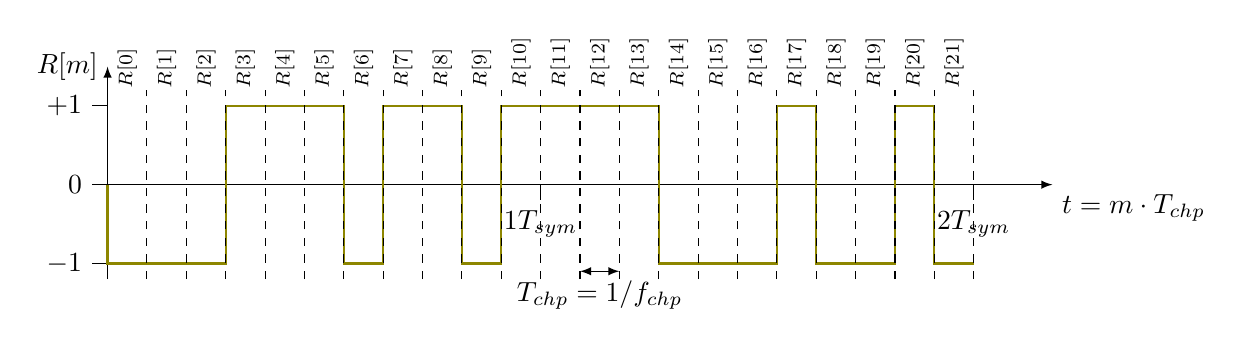
\begin{tikzpicture}
		\draw[-latex] (0,0) -- (12,0) node[below right, align=left]{$t = m \cdot T_{chp}$};
		\draw[-latex] (0,-1.2) -- (0,1.5) node[left, align=right]{$R[m]$};
		\foreach \y in {-1, 0, +1}{
			\draw (0,\y) -- (-0.2,\y) node[left,align=right]{$\y$};
		}
		\foreach \x/\t in {5.5/1, 11/2}{
			\draw (\x,0) -- (\x,-0.2) node[below,align=center]{$\t T_{sym}$};
		}
		
		\draw[olive,thick] (0,0) \foreach \n/\d in {0/-1, 1/+1} {
			\foreach \l/\c in {0/+1, 1/+1, 2/+1, 3/-1, 4/-1, 5/-1, 6/+1, 7/-1, 8/-1, 9/+1, 10/-1}{
				-- ({(\n*5.5)+(\l*0.5)},{\c*\d}) -- ({(\n*5.5)+(\l*0.5+0.5)},{\c*\d})
			}
		};
		
		%\draw[dashed] (5.5,-1.2) -- (5.5,1.2);
		%\draw[dashed] (11,-1.2) -- (11,1.2);
		\foreach \m in {0,1,...,21}{
			\node[anchor=west,rotate=90,align=center] at({(\m*0.5)+0.25},1.1) {\scriptsize $R[\m]$};
			\draw[dashed] ({(\m+1)*0.5},-1.2) -- ({(\m+1)*0.5},1.2);
		}
		
		\draw[latex-latex] (6,-1.1) -- node[midway,below,align=center]{$T_{chp} = 1/f_{chp}$} (6.5,-1.1);
		\end{tikzpicture}
	}
	
	\subfloat[Code chips]{
		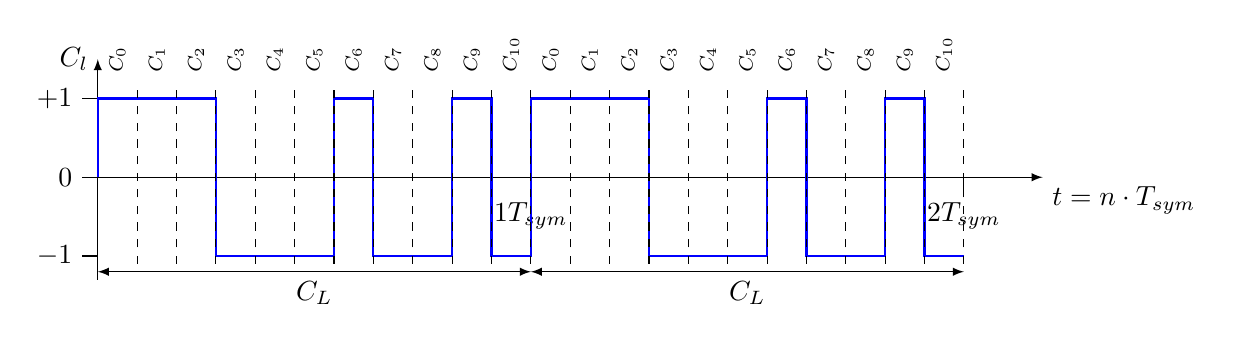
\begin{tikzpicture}
		\draw[-latex] (0,0) -- (12,0) node[below right, align=left]{$t = n \cdot T_{sym}$};
		\draw[-latex] (0,-1.3) -- (0,1.5) node[left, align=right]{$C_l$};
		\foreach \y in {-1, 0, +1}{
			\draw (0,\y) -- (-0.2,\y) node[left,align=right]{$\y$};
		}
		\foreach \x/\t in {5.5/1, 11/2}{
			\draw (\x,0) -- (\x,-0.2) node[below,align=center]{$\t T_{sym}$};
		}
		
		\draw[blue,thick] (0,0) \foreach \n in {0, 1} {
			\foreach \l/\c in {0/+1, 1/+1, 2/+1, 3/-1, 4/-1, 5/-1, 6/+1, 7/-1, 8/-1, 9/+1, 10/-1}{
				-- ({(\n*5.5)+(\l*0.5)},\c) -- ({(\n*5.5)+(\l*0.5+0.5)},\c)
			}
		};
		
		%\draw[dashed] (5.5,-1.2) -- (5.5,1.2);
		%\draw[dashed] (11,-1.2) -- (11,1.2);
		\foreach \n in {0, 1} {
			\foreach \l in {0,1,...,10}{
				\node[anchor=west,rotate=90,align=center] at({((\n*11+\l)*0.5)+0.25},1.2) {\scriptsize $C_{\l}$};
				\draw[dashed] ({((\n*11+\l)+1)*0.5},-1.1) -- ({((\n*11+\l)+1)*0.5},1.2);
			}
		}
		
		\foreach \x/\n in {0/0, 5.5/1}{
			\draw[latex-latex] (\x,-1.2) -- node[midway,below,align=center]{$\vect{C}_L$} ({\x+5.5},-1.2);
		}
		\end{tikzpicture}
	}
	
	\subfloat[Accumulation of cross-correlation. The grey circles are the sampling (detection) and reset points.]{
		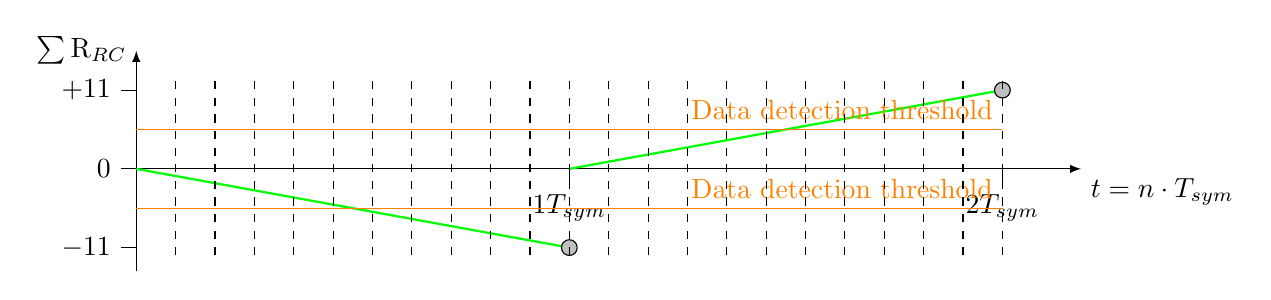
\begin{tikzpicture}
		\draw[-latex] (0,0) -- (12,0) node[below right, align=left]{$t = n \cdot T_{sym}$};
		\draw[-latex] (0,-1.3) -- (0,1.5) node[left, align=right]{$\sum \mathrm{R}_{RC}$};
		\foreach \y/\v in {-1/-11, 0, +1/+11}{
			\draw (0,\y) -- (-0.2,\y) node[left,align=right]{$\v$};
		}
		\foreach \x/\t in {5.5/1, 11/2}{
			\draw (\x,0) -- (\x,-0.2) node[below,align=center]{$\t T_{sym}$};
		}
		
		\draw[green,thick] (0,0) -- ++(5.5,-1);
		\draw[fill=gray!50,draw] (5.5,-1) ++(0:0.1) arc(0:360:0.1);
		\draw[green,thick] (5.5,0) -- ++(5.5,1);
		\draw[fill=gray!50,draw] (11,1) ++(0:0.1) arc(0:360:0.1);
		
		\foreach \y in {-0.5,0.5}{
			\draw[orange] (0,\y) -- (11,\y) node[anchor=south east,align=right]{Data detection threshold};
		}
		
		%\draw[dashed] (5.5,-1.2) -- (5.5,1.2);
		%\draw[dashed] (11,-1.2) -- (11,1.2);
		\foreach \n in {0, 1} {
			\foreach \l in {0,1,...,10}{
				%\node[anchor=west,rotate=90,align=center] at({((\n*11+\l)*0.5)+0.25},1.2) {\scriptsize $C_{\l}$};
				\draw[dashed] ({((\n*11+\l)+1)*0.5},-1.1) -- ({((\n*11+\l)+1)*0.5},1.2);
			}
		}
		\end{tikzpicture}
	}
	
	\subfloat[Data symbols]{
		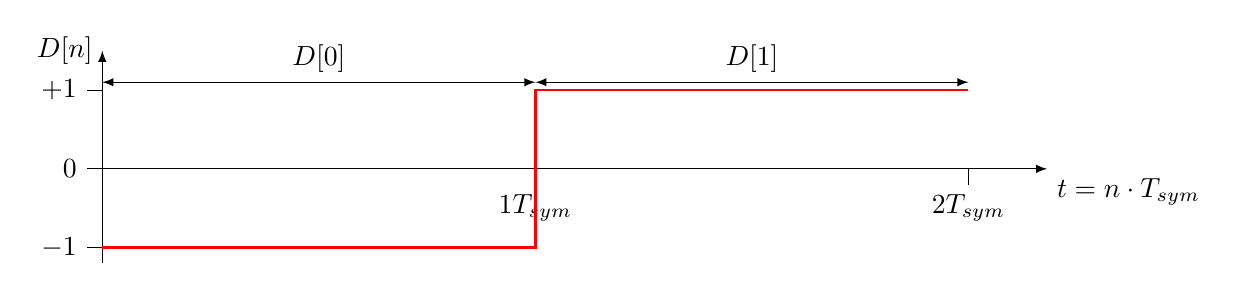
\begin{tikzpicture}
		\draw[-latex] (0,0) -- (12,0) node[below right, align=left]{$t = n \cdot T_{sym}$};
		\draw[-latex] (0,-1.2) -- (0,1.5) node[left, align=right]{$D[n]$};
		\foreach \y in {-1, 0, +1}{
			\draw (0,\y) -- (-0.2,\y) node[left,align=right]{$\y$};
		}
		\foreach \x/\t in {5.5/1, 11/2}{
			\draw (\x,0) -- (\x,-0.2) node[below,align=center]{$\t T_{sym}$};
		}
		
		\foreach \x/\n in {0/0, 5.5/1}{
			\draw[latex-latex] (\x,1.1) -- node[midway,above,align=center]{$D[\n]$} ({\x+5.5},1.1);
		}
		
		\draw[red,thick] (0,-1) -- (5.5,-1) -- (5.5,1) -- (11,1);
		\end{tikzpicture}
	}
	
	\caption{Despreading of a noise-free \acs{DSSS} signal}
\end{figure}

\begin{figure}[H]
	\centering
	
	\subfloat[Received chips]{
		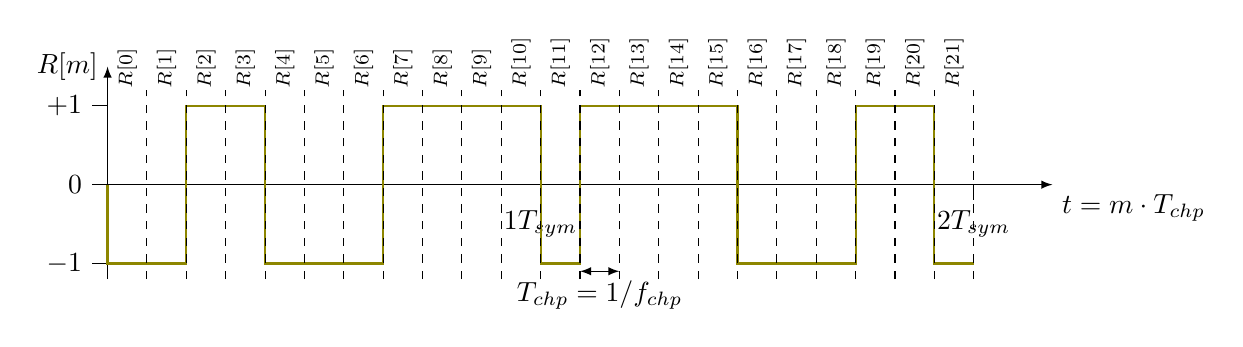
\begin{tikzpicture}
		\draw[-latex] (0,0) -- (12,0) node[below right, align=left]{$t = m \cdot T_{chp}$};
		\draw[-latex] (0,-1.2) -- (0,1.5) node[left, align=right]{$R[m]$};
		\foreach \y in {-1, 0, +1}{
			\draw (0,\y) -- (-0.2,\y) node[left,align=right]{$\y$};
		}
		\foreach \x/\t in {5.5/1, 11/2}{
			\draw (\x,0) -- (\x,-0.2) node[below,align=center]{$\t T_{sym}$};
		}
		
		\draw[olive,thick] (0,0) \foreach \m/\r in {0/-1, 1/-1, 2/+1, 3/+1, 4/-1, 5/-1, 6/-1, 7/+1, 8/+1, 9/+1, 10/+1, 11/-1, 12/+1, 13/+1, 14/+1, 15/+1, 16/-1, 17/-1, 18/-1, 19/+1, 20/+1, 21/-1}{
				-- ({(\m*0.5)},{\r}) -- ({(\m*0.5+0.5)},{\r})
		};
		
		%\draw[dashed] (5.5,-1.2) -- (5.5,1.2);
		%\draw[dashed] (11,-1.2) -- (11,1.2);
		\foreach \m in {0,1,...,21}{
			\node[anchor=west,rotate=90,align=center] at({(\m*0.5)+0.25},1.1) {\scriptsize $R[\m]$};
			\draw[dashed] ({(\m+1)*0.5},-1.2) -- ({(\m+1)*0.5},1.2);
		}
		
		\draw[latex-latex] (6,-1.1) -- node[midway,below,align=center]{$T_{chp} = 1/f_{chp}$} (6.5,-1.1);
		\end{tikzpicture}
	}
	
	\subfloat[Code chips]{
		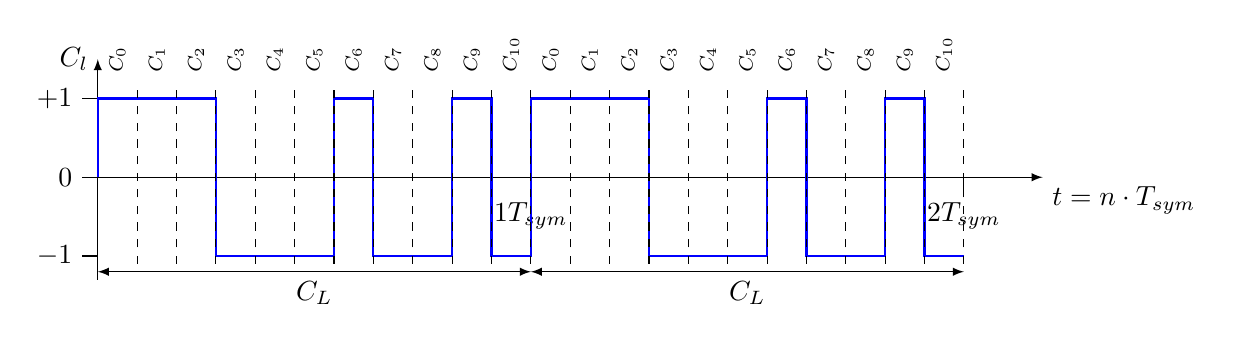
\begin{tikzpicture}
		\draw[-latex] (0,0) -- (12,0) node[below right, align=left]{$t = n \cdot T_{sym}$};
		\draw[-latex] (0,-1.3) -- (0,1.5) node[left, align=right]{$C_l$};
		\foreach \y in {-1, 0, +1}{
			\draw (0,\y) -- (-0.2,\y) node[left,align=right]{$\y$};
		}
		\foreach \x/\t in {5.5/1, 11/2}{
			\draw (\x,0) -- (\x,-0.2) node[below,align=center]{$\t T_{sym}$};
		}
		
		\draw[blue,thick] (0,0) \foreach \n in {0, 1} {
			\foreach \l/\c in {0/+1, 1/+1, 2/+1, 3/-1, 4/-1, 5/-1, 6/+1, 7/-1, 8/-1, 9/+1, 10/-1}{
				-- ({(\n*5.5)+(\l*0.5)},\c) -- ({(\n*5.5)+(\l*0.5+0.5)},\c)
			}
		};
		
		%\draw[dashed] (5.5,-1.2) -- (5.5,1.2);
		%\draw[dashed] (11,-1.2) -- (11,1.2);
		\foreach \n in {0, 1} {
			\foreach \l in {0,1,...,10}{
				\node[anchor=west,rotate=90,align=center] at({((\n*11+\l)*0.5)+0.25},1.2) {\scriptsize $C_{\l}$};
				\draw[dashed] ({((\n*11+\l)+1)*0.5},-1.1) -- ({((\n*11+\l)+1)*0.5},1.2);
			}
		}
		
		\foreach \x/\n in {0/0, 5.5/1}{
			\draw[latex-latex] (\x,-1.2) -- node[midway,below,align=center]{$\vect{C}_L$} ({\x+5.5},-1.2);
		}
		\end{tikzpicture}
	}
	
	\subfloat[Accumulation of cross-correlation. The grey circles are the sampling (detection) and reset points.]{
		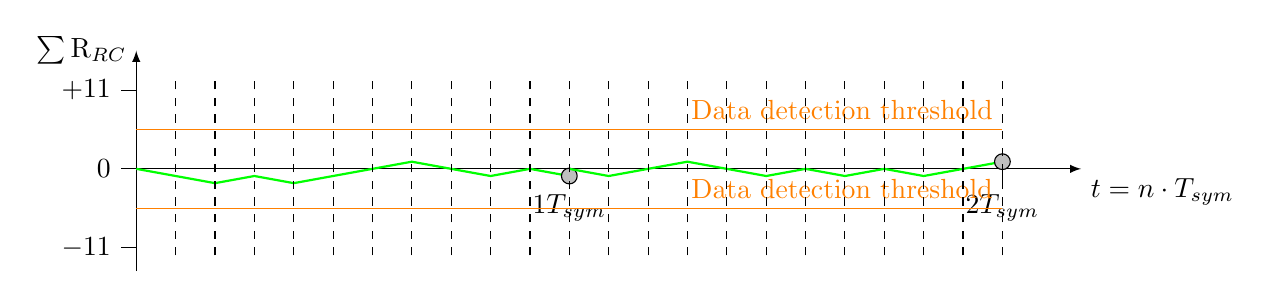
\begin{tikzpicture}
		\draw[-latex] (0,0) -- (12,0) node[below right, align=left]{$t = n \cdot T_{sym}$};
		\draw[-latex] (0,-1.3) -- (0,1.5) node[left, align=right]{$\sum \mathrm{R}_{RC}$};
		\foreach \y/\v in {-1/-11, 0, +1/+11}{
			\draw (0,\y) -- (-0.2,\y) node[left,align=right]{$\v$};
		}
		\foreach \x/\t in {5.5/1, 11/2}{
			\draw (\x,0) -- (\x,-0.2) node[below,align=center]{$\t T_{sym}$};
		}
		
		\draw[green,thick] (0,0) \foreach \v in {-1,-1,+1,-1,+1,+1,+1,-1,-1,+1,-1}{ -- ++(0.5,{\v/11})};
		\draw[fill=gray!50,draw] (5.5,{-1/11}) ++(0:0.1) arc(0:360:0.1);
		\draw[green,thick] (5.5,0) \foreach \v in {-1,+1,+1,-1,-1,+1,-1,+1,-1,+1,+1}{ -- ++(0.5,{\v/11})};
		\draw[fill=gray!50,draw] (11,{+1/11}) ++(0:0.1) arc(0:360:0.1);
		
		\foreach \y in {-0.5,0.5}{
			\draw[orange] (0,\y) -- (11,\y) node[anchor=south east,align=right]{Data detection threshold};
		}
		
		%\draw[dashed] (5.5,-1.2) -- (5.5,1.2);
		%\draw[dashed] (11,-1.2) -- (11,1.2);
		\foreach \n in {0, 1} {
			\foreach \l in {0,1,...,10}{
				%\node[anchor=west,rotate=90,align=center] at({((\n*11+\l)*0.5)+0.25},1.2) {\scriptsize $C_{\l}$};
				\draw[dashed] ({((\n*11+\l)+1)*0.5},-1.1) -- ({((\n*11+\l)+1)*0.5},1.2);
			}
		}
		\end{tikzpicture}
	}
	
	\subfloat[Data symbols]{
		\begin{tikzpicture}
		\draw[-latex] (0,0) -- (12,0) node[below right, align=left]{$t = n \cdot T_{sym}$};
		\draw[-latex] (0,-1.2) -- (0,1.5) node[left, align=right]{$D[n]$};
		\foreach \y in {-1, 0, +1}{
			\draw (0,\y) -- (-0.2,\y) node[left,align=right]{$\y$};
		}
		\foreach \x/\t in {5.5/1, 11/2}{
			\draw (\x,0) -- (\x,-0.2) node[below,align=center]{$\t T_{sym}$};
		}
		
		\draw[red,thick] (0,0) -- node[midway,above,align=center]{No data} (11,0);
		\end{tikzpicture}
	}
	
	\caption{\acs{DSSS} despreading of pure noise}
\end{figure}

\begin{figure}[H]
	\centering
	
	\subfloat[Received chips]{
		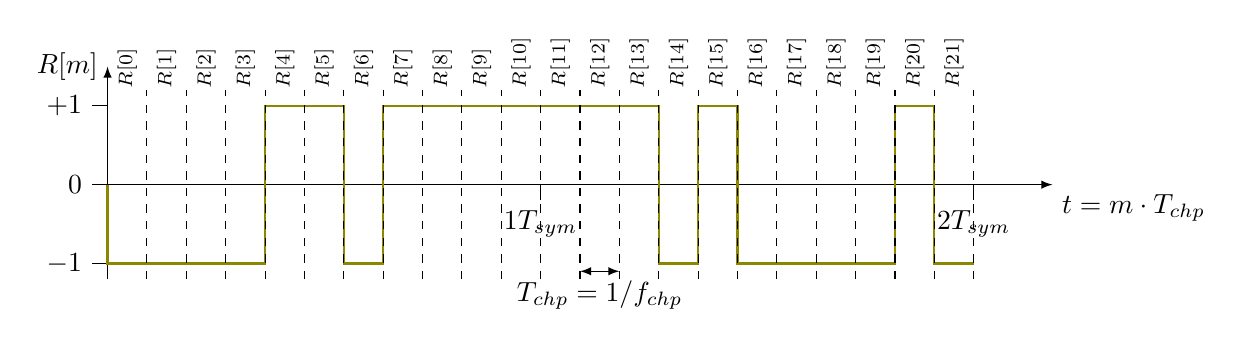
\begin{tikzpicture}
		\draw[-latex] (0,0) -- (12,0) node[below right, align=left]{$t = m \cdot T_{chp}$};
		\draw[-latex] (0,-1.2) -- (0,1.5) node[left, align=right]{$R[m]$};
		\foreach \y in {-1, 0, +1}{
			\draw (0,\y) -- (-0.2,\y) node[left,align=right]{$\y$};
		}
		\foreach \x/\t in {5.5/1, 11/2}{
			\draw (\x,0) -- (\x,-0.2) node[below,align=center]{$\t T_{sym}$};
		}
	
		\draw[olive,thick] (0,0) \foreach \m/\r in {0/-1, 1/-1, 2/-1, 3/-1, 4/+1, 5/+1, 6/-1, 7/+1, 8/+1, 9/+1, 10/+1, 11/+1, 12/+1, 13/+1, 14/-1, 15/+1, 16/-1, 17/-1, 18/-1, 19/-1, 20/+1, 21/-1}{
			-- ({(\m*0.5)},{\r}) -- ({(\m*0.5+0.5)},{\r})
		};
		
		%\draw[dashed] (5.5,-1.2) -- (5.5,1.2);
		%\draw[dashed] (11,-1.2) -- (11,1.2);
		\foreach \m in {0,1,...,21}{
			\node[anchor=west,rotate=90,align=center] at({(\m*0.5)+0.25},1.1) {\scriptsize $R[\m]$};
			\draw[dashed] ({(\m+1)*0.5},-1.2) -- ({(\m+1)*0.5},1.2);
		}
		
		\draw[latex-latex] (6,-1.1) -- node[midway,below,align=center]{$T_{chp} = 1/f_{chp}$} (6.5,-1.1);
		\end{tikzpicture}
	}
	
	\subfloat[Code chips]{
		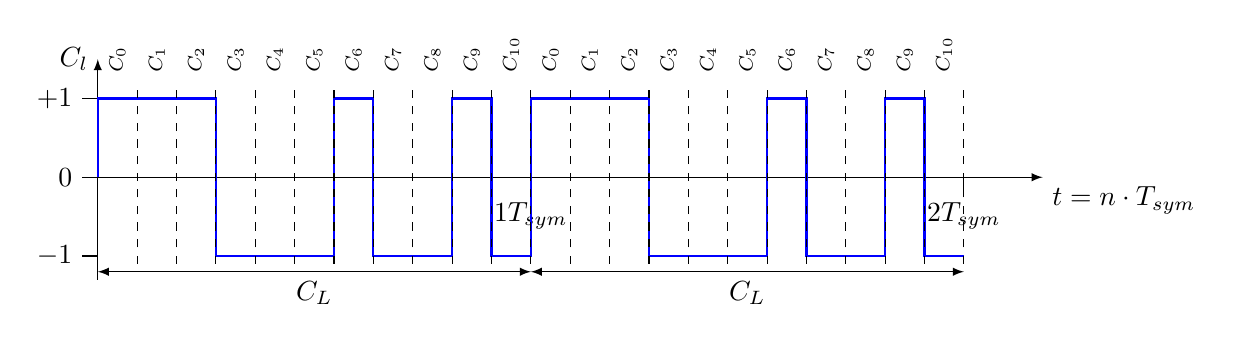
\begin{tikzpicture}
		\draw[-latex] (0,0) -- (12,0) node[below right, align=left]{$t = n \cdot T_{sym}$};
		\draw[-latex] (0,-1.3) -- (0,1.5) node[left, align=right]{$C_l$};
		\foreach \y in {-1, 0, +1}{
			\draw (0,\y) -- (-0.2,\y) node[left,align=right]{$\y$};
		}
		\foreach \x/\t in {5.5/1, 11/2}{
			\draw (\x,0) -- (\x,-0.2) node[below,align=center]{$\t T_{sym}$};
		}
		
		\draw[blue,thick] (0,0) \foreach \n in {0, 1} {
			\foreach \l/\c in {0/+1, 1/+1, 2/+1, 3/-1, 4/-1, 5/-1, 6/+1, 7/-1, 8/-1, 9/+1, 10/-1}{
				-- ({(\n*5.5)+(\l*0.5)},\c) -- ({(\n*5.5)+(\l*0.5+0.5)},\c)
			}
		};
		
		%\draw[dashed] (5.5,-1.2) -- (5.5,1.2);
		%\draw[dashed] (11,-1.2) -- (11,1.2);
		\foreach \n in {0, 1} {
			\foreach \l in {0,1,...,10}{
				\node[anchor=west,rotate=90,align=center] at({((\n*11+\l)*0.5)+0.25},1.2) {\scriptsize $C_{\l}$};
				\draw[dashed] ({((\n*11+\l)+1)*0.5},-1.1) -- ({((\n*11+\l)+1)*0.5},1.2);
			}
		}
		
		\foreach \x/\n in {0/0, 5.5/1}{
			\draw[latex-latex] (\x,-1.2) -- node[midway,below,align=center]{$\vect{C}_L$} ({\x+5.5},-1.2);
		}
		\end{tikzpicture}
	}
	
	\subfloat[Accumulation of cross-correlation. The grey circles are the sampling (detection) and reset points.]{
		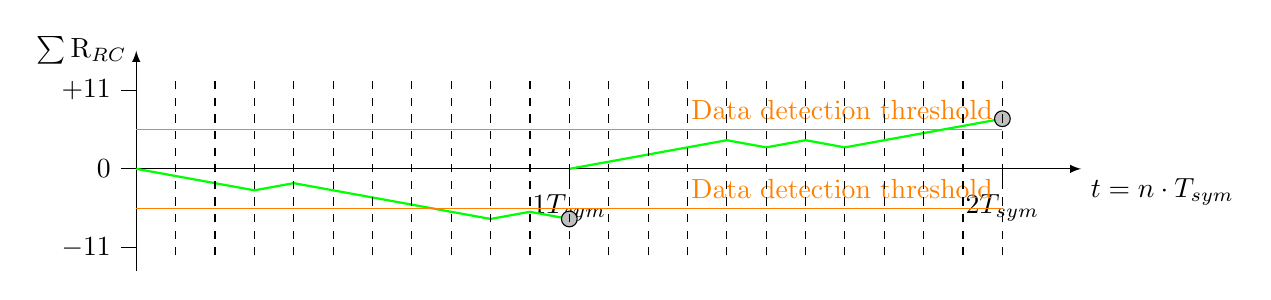
\begin{tikzpicture}
		\draw[-latex] (0,0) -- (12,0) node[below right, align=left]{$t = n \cdot T_{sym}$};
		\draw[-latex] (0,-1.3) -- (0,1.5) node[left, align=right]{$\sum \mathrm{R}_{RC}$};
		\foreach \y/\v in {-1/-11, 0, +1/+11}{
			\draw (0,\y) -- (-0.2,\y) node[left,align=right]{$\v$};
		}
		\foreach \x/\t in {5.5/1, 11/2}{
			\draw (\x,0) -- (\x,-0.2) node[below,align=center]{$\t T_{sym}$};
		}
		
		\draw[green,thick] (0,0) \foreach \v in {-1,-1,-1,+1,-1,-1,-1,-1,-1,+1,-1}{ -- ++(0.5,{\v/11})};
		\draw[fill=gray!50,draw] (5.5,{-7/11}) ++(0:0.1) arc(0:360:0.1);
		\draw[green,thick] (5.5,0) \foreach \v in {+1,+1,+1,+1,-1,+1,-1,+1,+1,+1,+1}{ -- ++(0.5,{\v/11})};
		\draw[fill=gray!50,draw] (11,{+7/11}) ++(0:0.1) arc(0:360:0.1);
		
		\foreach \y in {-0.5,0.5}{
			\draw[orange] (0,\y) -- (11,\y) node[anchor=south east,align=right]{Data detection threshold};
		}
		
		%\draw[dashed] (5.5,-1.2) -- (5.5,1.2);
		%\draw[dashed] (11,-1.2) -- (11,1.2);
		\foreach \n in {0, 1} {
			\foreach \l in {0,1,...,10}{
				%\node[anchor=west,rotate=90,align=center] at({((\n*11+\l)*0.5)+0.25},1.2) {\scriptsize $C_{\l}$};
				\draw[dashed] ({((\n*11+\l)+1)*0.5},-1.1) -- ({((\n*11+\l)+1)*0.5},1.2);
			}
		}
		\end{tikzpicture}
	}
	
	\subfloat[Data symbols]{
		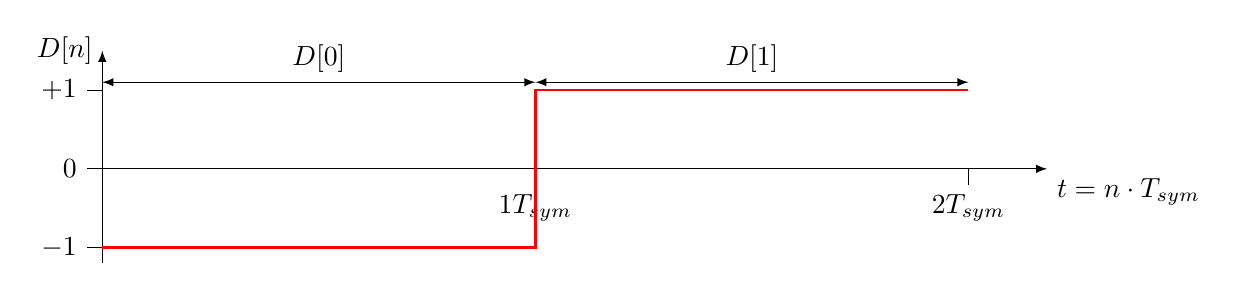
\begin{tikzpicture}
		\draw[-latex] (0,0) -- (12,0) node[below right, align=left]{$t = n \cdot T_{sym}$};
		\draw[-latex] (0,-1.2) -- (0,1.5) node[left, align=right]{$D[n]$};
		\foreach \y in {-1, 0, +1}{
			\draw (0,\y) -- (-0.2,\y) node[left,align=right]{$\y$};
		}
		\foreach \x/\t in {5.5/1, 11/2}{
			\draw (\x,0) -- (\x,-0.2) node[below,align=center]{$\t T_{sym}$};
		}
		
		\foreach \x/\n in {0/0, 5.5/1}{
			\draw[latex-latex] (\x,1.1) -- node[midway,above,align=center]{$D[\n]$} ({\x+5.5},1.1);
		}
		
		\draw[red,thick] (0,-1) -- (5.5,-1) -- (5.5,1) -- (11,1);
		\end{tikzpicture}
	}
	
	\caption[Despreading of a noisy \acs{DSSS} signal]{Despreading of a noisy \acs{DSSS} signal. The noise shows up as flipped chips in the received chip sequence.}
\end{figure}


\subsubsection{Processing Gain}

In fact, the \ac{DSSS} despreading consists of
\begin{itemize}
	\item \textbf{Down-sampling}: The received and cross-correlated chips are down-sampled by $L$, the length of the \emph{spreading code} length.
	\item \textbf{Filtering}: The accumulator is in fact a \ac{FIR} low-pass filter.
\end{itemize}

The \emph{down-sampling} provides a \index{processing gain} \textbf{processing gain} of $L$.
\begin{itemize}
	\item The processing gain improves the \ac{SNR} by $+ \SI{10}{dB} \cdot \log_{10} \left(L\right)$.
	\item The spread spectrum signal is more immune against noise.
\end{itemize}

\begin{fact}
	Despreading of spread spectrum signals provides a processing gain.
\end{fact}

The processing gain is not only limited to wide-band (\ac{AWGN}, thermal, quantization, etc. noise). Narrow-band disturbances are suppressed as long as they are uncorrelated with the \emph{spreading code}. The cross-correlation has only a peak when the code matches and will be low if the code does not match. So, all uncorrelated superimposed signals can be removed. This is the strength of spread spectrum techniques.

\begin{figure}[H]
	\centering
	
	\subfloat[\acs{PSD} of the received signal \textbf{before} despreading]{
		\centering
		\begin{tikzpicture}
			\begin{axis}[
					height={0.15\textheight},
					width=0.8\linewidth,
					scale only axis,
					xlabel={$\omega$},
					ylabel={$|\mathrm{S}_{RR}|$},
					%grid style={line width=.6pt, color=lightgray},
					%grid=both,
					grid=none,
					legend pos=north east,
					axis y line=middle,
					axis x line=middle,
					every axis x label/.style={
						at={(ticklabel* cs:1.05)},
						anchor=north,
					},
					every axis y label/.style={
						at={(ticklabel* cs:1.05)},
						anchor=east,
					},
					xmin=0,
					xmax=10.5,
					ymin=0,
					ymax=1.2,
					xtick={0},
					xticklabels={0},
					ytick={0},
					axis x discontinuity=parallel,
				]
					\addplot[red, smooth] coordinates {(2,0) (2.5,0.01) (3,0.05) (5,0.05) (7,0.05) (7.5,0.01) (8,0)};
					\addlegendentry{Spread spectrum signal};
					\addplot[blue, smooth] coordinates {(4.6,0) (4.7,0.02) (4.8,0.2) (4.9,0.71) (5,1) (5.1,0.71) (5.2,0.2) (5.3,0.02) (5.4,0)};
					\addlegendentry{Narrow-band noise};
					\addplot[green, smooth] coordinates {(0,0.03) (10,0.03)};
					\addlegendentry{Wide-band noise};
			\end{axis}
		\end{tikzpicture}
	}

	\subfloat[\acs{PSD} of the received signal \textbf{after} despreading]{
		\centering
		\begin{tikzpicture}
			\begin{axis}[
				height={0.15\textheight},
				width=0.8\linewidth,
				scale only axis,
				xlabel={$\omega$},
				ylabel={$|\mathrm{S}_{\tilde{R}\tilde{R}}|$},
				%grid style={line width=.6pt, color=lightgray},
				%grid=both,
				grid=none,
				legend pos=north east,
				axis y line=middle,
				axis x line=middle,
				every axis x label/.style={
					at={(ticklabel* cs:1.05)},
					anchor=north,
				},
				every axis y label/.style={
					at={(ticklabel* cs:1.05)},
					anchor=east,
				},
				xmin=0,
				xmax=10.5,
				ymin=0,
				ymax=1.2,
				xtick={0},
				xticklabels={0},
				ytick={0},
				axis x discontinuity=parallel,
			]
				\addplot[red, smooth] coordinates {(4.6,0) (4.7,0.02) (4.8,0.2) (4.9,0.71) (5,1) (5.1,0.71) (5.2,0.2) (5.3,0.02) (5.4,0)};
				\addlegendentry{Spread spectrum signal};
				\addplot[blue, smooth] coordinates {(2,0) (2.5,0.01) (3,0.05) (5,0.05) (7,0.05) (7.5,0.01) (8,0)};
				\addlegendentry{Narrow-band noise};
				\addplot[green, smooth] coordinates {(0,0.03) (10,0.03)};
				\addlegendentry{Wide-band noise};
				
				\draw[latex-latex] (axis cs:4,0.05) -- node[midway,left,align=right]{Improved \acs{SNR}} (axis cs:4,1);
			\end{axis}
		\end{tikzpicture}
	}

	\caption[Processing gain of despreading]{Processing gain of despreading. The received signal is composed of the spread spectrum signal and two noise components (narrow-band and wide-band noise). After despreading the spread spectrum signal is reconstructed while both (uncorrelated) narrow-band and wide-band noise are attenuated. Despreading spreads the \acs{PSD} of the narrow-band noise, while the \ac{PSD} of the wide-band noise is not changed. The narrow-band noise does not interfere, even if it at the centre frequency of the spread spectrum signal like in this case.}
\end{figure}

\section{Multi-carrier Modulation}

Multi-carrier modulation is a spread spectrum technique, which does not only increase the bandwidth whilst keeping the data rate constant. Multi-carrier modulation is related to \ac{FHSS}, but does not implement a hopping scheme. Instead, all sub-band are used, to transmit $M$ data streams parallelly.

\begin{itemize}
	\item The (serial) sequence of data symbols is parallelized.
	\item The $M$ parallel symbol streams are then modulated independently.
	\item Each modulated symbol stream is then transmitted in another sub-band.
\end{itemize}

\begin{figure}[H]
	\centering
	\begin{adjustbox}{scale=0.8}
		\begin{circuitikz}
			\node[draw,block,minimum height=6cm](SP){Serial-to-\\ parallel};
			\node[adder,right=8cm of SP](Add){};
			
			\draw[-o] (SP.west) node[inputarrow]{} -- ++(-1cm,0) node[left,align=right]{Data stream $\vect{D}$};
			
			\foreach \n/\y in {1/2.5, 2/1, M/-2.5}{
				\draw ([yshift={\y cm}]SP.east) -- ++(1cm,0) node[inputarrow]{} node[draw,block,anchor=west](Mod\n){Modulator \n};
				\draw (Mod\n.east) -- ++(1cm,0) node[inputarrow]{} node[mixer,anchor=west](Mix\n){};
			}
		
			\node[above=5mm of Mix1,align=center]{Sub-band\\ mixers};
		
			\draw (Mix1.east) -| (Add.north) node[inputarrow,rotate=-90]{};
			\draw (Mix2.east) -| (Add.north);
			\draw (MixM.east) -| (Add.south) node[inputarrow,rotate=90]{};
			
			\draw[draw=none] (Mod2.south) -- node[midway]{$\vdots$} (ModM.north);
		
			\draw (Add.east) -- ++(1cm,0) node[inputarrow]{} node[right,align=left]{Multi-carrier\\ signal};
		\end{circuitikz}
	\end{adjustbox}
	\caption{Multi-carrier modulator}
\end{figure}

\begin{itemize}
	\item If the rate of the input symbols is $f_{sym}$, the symbol rate in each of the $M$ parallel streams is $f_{sym,M}$. \nomenclature[Sf]{$f_{sym,M}$}{Symbol rate in one of the $M$ sub-bands}
	\begin{equation}
		f_{sym,M} = \frac{f_{sym}}{M}
	\end{equation}
	\item The symbol period in each sub-band is $M$ times longer. \nomenclature[Sf]{$T_{sym,M}$}{Symbol period in one of the $M$ sub-bands}
	\begin{equation}
		T_{sym,M} = M \cdot T_{sym}
	\end{equation}
	\item The bandwidth of one sub-band is approximately $\Delta f_{sub} \approx f_{sym,M}$.
	\item The total bandwidth $\Delta f_{MC}$ of all sub-bands together is approximately $\Delta f_{MC} = M \cdot \Delta f_{sub} \approx f_{sym}$.
	\item The duration of one transmitted symbol is $T_{sym,M}$.
	\item the \emph{time-bandwidth product} is
	\begin{equation}
		\Delta f_{MC} \cdot T_{sym,M} = M \gg 1
	\end{equation}
	The condition for a spread spectrum signal is fulfilled.
\end{itemize}

\begin{figure}[H]
	\centering
	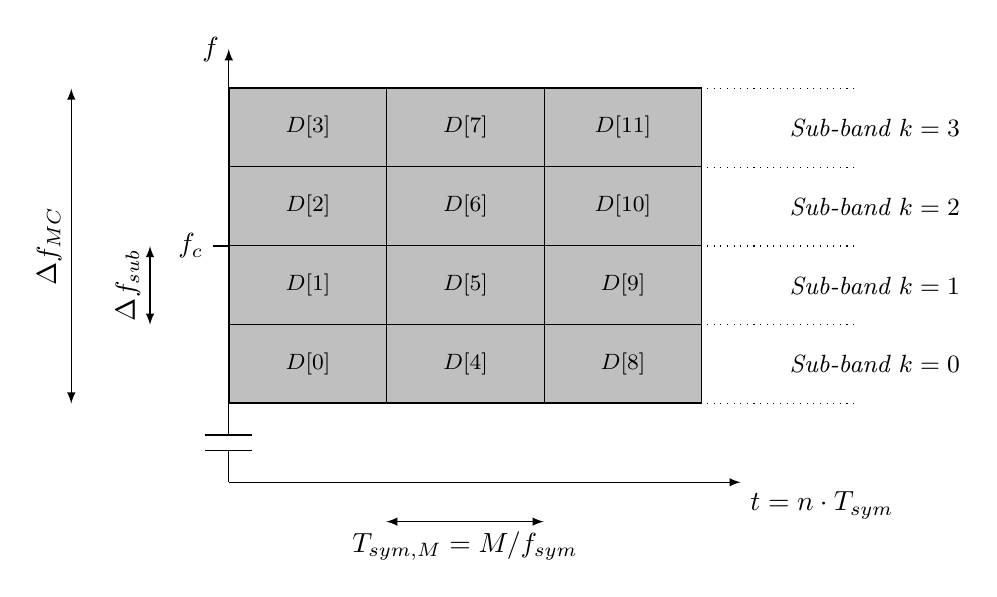
\begin{tikzpicture}[x=1cm,y=1cm]
		\draw[-latex] (0,0) -- (6.5,0) node[below right, align=left]{$t = n \cdot T_{sym}$};
		\draw[-latex] (0,0) -- (0,0.4) (0,0.6) -- (0,5.5) node[left, align=right]{$f$};
		\draw (-0.3,0.4) -- (0.3,0.4);
		\draw (-0.3,0.6) -- (0.3,0.6);
		
		\draw (0,3) -- (-0.2,3) node[left,align=right]{$f_c$};
		\draw[latex-latex] (-1,2) -- node[midway,left,align=center,anchor=south,rotate=90]{$\Delta f_{sub}$} (-1,3);
		\draw[latex-latex] (-2,1) -- node[midway,left,align=center,anchor=south,rotate=90]{$\Delta f_{MC}$} (-2,5);
		\draw[latex-latex] (2,-0.5) -- node[midway,below,align=center]{$T_{sym,M} = M/f_{sym}$} (4,-0.5);
		
		\foreach \k in {0, 1, 2, 3}{
			\draw[dotted] (0,{\k+1}) -- (8,{\k+1});
			\node[right,align=left] at(7,{\k+1.5}) {\small\itshape Sub-band $k = \k$};
		}
		\draw[dotted] (0,5) -- (8,5);
		
		\foreach \n/\x/\k in {0/0/0, 1/0/1, 2/0/2, 3/0/3, 4/1/0, 5/1/1, 6/1/2, 7/1/3, 8/2/0, 9/2/1, 10/2/2, 11/2/3}{
			\node[fill=gray!50, draw=black, minimum height=1cm, minimum width=2cm, anchor=south west] at({\x*2},{\k+1}) {\footnotesize $D[\n]$};
		}
	\end{tikzpicture}
	\caption[Time-frequency plot: distribution of symbols in an $M$-ary multi-carrier modulation (with $M = 4$)]{Time-frequency plot: distribution of symbols in an $M$-ary multi-carrier modulation (with $M = 4$). $M$ symbols can be transmitted parallelly. The symbol rate is reduced proportionally.}
	\label{fig:ch07:mulcarr_mod_spectrum}
\end{figure}

\subsection{Inter-Carrier Interference}

The \emph{\ac{ISI}} was an issue in the time-domain.
\begin{itemize}
	\item Neighbouring symbols interfered if no guard interval was inserted.
	\item The reason was the band limitation of the symbols, which flattened the ideal, rectangular slopes of the symbols in the time-domain.
\end{itemize}

Due to the duality of time-domain and frequency-domain, an analogous problem arises in the frequency domain -- the \index{inter-carrier interference} \textbf{inter-carrier interference}.
\begin{itemize}
	\item Symbols are assumed to be ideal. They have a rectangular shape.
	\item Their Fourier transform is a sinc-function, whose \ac{PSD} spreads across the infinite frequency range.
	\item The side lobes of neighbouring sinc-functions would overlap. A symbol in one sub-band would interfere with its neighbouring sub-bands.
	\item \textbf{A \emph{guard band} must be inserted to reduce the interference.}
\end{itemize}

\begin{figure}[H]
	\centering
	\begin{tikzpicture}
		\begin{axis}[
			height={0.15\textheight},
			width=0.7\linewidth,
			scale only axis,
			xlabel={$f$},
			ylabel={Sub-bands},
			%grid style={line width=.6pt, color=lightgray},
			%grid=both,
			grid=none,
			legend pos=outer north east,
			axis y line=middle,
			axis x line=middle,
			every axis x label/.style={
				at={(ticklabel* cs:1.05)},
				anchor=north,
			},
			every axis y label/.style={
				at={(ticklabel* cs:1.05)},
				anchor=east,
			},
			xmin=-0.5,
			xmax=8.5,
			ymin=0,
			ymax=1.7,
			%xtick={0,0.125,...,1},
			%xticklabels={$- \omega_S$, $- \frac{\omega_S}{2}$, $0$, $\frac{\omega_S}{2}$, $\omega_S$},
			%ytick={0},
		]
			\addplot[blue,smooth] coordinates {(-1.5,0) (0,0.5) (0.5,0.85) (1,1) (1.5,0.85) (2,0.5) (3.5,0)};
			\addplot[red,smooth] coordinates {(0.5,0) (2,0.5) (2.5,0.85) (3,1) (3.5,0.85) (4,0.5) (5.5,0)};
			\addplot[green,smooth] coordinates {(2.5,0) (4,0.5) (4.5,0.85) (5,1) (5.5,0.85) (6,0.5) (7.5,0)};
			\addplot[olive,smooth] coordinates {(4.5,0) (6,0.5) (6.5,0.85) (7,1) (7.5,0.85) (8,0.5) (9.5,0)};
			
			\draw[dashed] (axis cs:2,0) -- (axis cs:2,1.2);
			\draw[dashed] (axis cs:4,0) -- (axis cs:4,1.2);
			\draw[latex-latex] (axis cs:2,1.1) -- node[midway,above,align=center]{Sub-band bandwidth $\Delta f_{sub}$} (axis cs:4,1.1);
		\end{axis}
	\end{tikzpicture}
	\caption{Neighbouring sub-bands interfering with each other and thereby causing inter-carrier interference}
\end{figure}

\begin{fact}
	All frequency-division spread spectrum techniques (\ac{FHSS} and multi-carrier) suffer from inter-carrier interference.
\end{fact}

A draw-back of inserting guard bands is the increased bandwidth of the whole multi-carrier signal.

\subsection{Orthogonal Frequency-Division Multiplex}

The increased bandwidth makes frequency-division spread spectrum techniques unattractive. Luckily, the inter-carrier interference issue can be mitigated without significantly increasing the bandwidth.
\begin{itemize}
	\item The sinc-function has a special property. It has \emph{zeros} at each $f = k \cdot \frac{1}{T_{sym,M}}$ (or as an angular freuqency $\omega = k \cdot \frac{2\pi}{T_{sym,M}}$) for all integer values except zero $k \in \mathbb{Z} \ \left\{0\right\}$.
	\item If the centre frequency (sub-carrier frequency) of the neighbouring sub-bands were at these zeros of the sinc-function, the inter-carrier interference would be minimal.
	\item Because the sub-carrier frequency is in a zero of the sin-function, \textbf{all sub-carriers are orthogonal}.
	\item This means that the optimal spacing between the carriers of the sub-bands $\Delta f_{sc-sc}$ (the \index{sub-carrier spacing} \textbf{sub-carrier spacing}) is
	\begin{equation}
		\Delta f_{sc-sc} = \frac{1}{T_{sym,M}} = f_{sym,M}
	\end{equation}%
	\nomenclature[Sf]{$\Delta f_{sc-sc}$}{Sub-carrier spacing in a multi-carrier system}
\end{itemize}

\begin{figure}[H]
	\centering
	\begin{tikzpicture}
		\begin{axis}[
			height={0.15\textheight},
			width=0.7\linewidth,
			scale only axis,
			xlabel={$f$},
			ylabel={\acs{OFDM} sub-bands},
			%grid style={line width=.6pt, color=lightgray},
			%grid=both,
			grid=none,
			legend pos=outer north east,
			axis y line=middle,
			axis x line=middle,
			every axis x label/.style={
				at={(ticklabel* cs:1.05)},
				anchor=north,
			},
			every axis y label/.style={
				at={(ticklabel* cs:1.05)},
				anchor=east,
			},
			xmin=-0.5,
			xmax=8.5,
			ymin=0,
			ymax=1.7,
			%xtick={0,0.125,...,1},
			%xticklabels={$- \omega_S$, $- \frac{\omega_S}{2}$, $0$, $\frac{\omega_S}{2}$, $\omega_S$},
			%ytick={0},
		]
			\addplot[blue,smooth,domain=0:8,samples=50] plot({\x},{(sinc(pi*(\x-3)))});
			\addplot[blue,smooth,domain=0:8,samples=50] plot({\x},{-(sinc(pi*(\x-3)))});
			\addplot[red,smooth,domain=0:8,samples=50] plot({\x},{(sinc(pi*(\x-4)))});
			\addplot[red,smooth,domain=0:8,samples=50] plot({\x},{-(sinc(pi*(\x-4)))});
			\addplot[green,smooth,domain=0:8,samples=50] plot({\x},{(sinc(pi*(\x-5)))});
			\addplot[green,smooth,domain=0:8,samples=50] plot({\x},{-(sinc(pi*(\x-5)))});
			\addplot[olive,smooth,domain=0:8,samples=50] plot({\x},{(sinc(pi*(\x-6)))});
			\addplot[olive,smooth,domain=0:8,samples=50] plot({\x},{-(sinc(pi*(\x-6)))});
			
			\draw[dashed] (axis cs:4,0) -- (axis cs:4,1.2);
			\draw[dashed] (axis cs:5,0) -- (axis cs:5,1.2);
			\draw[latex-latex] (axis cs:4,1.1) -- node[midway,above,align=center]{Sub-carrier spacing $\Delta f_{sc-sc}$} (axis cs:5,1.1);
		\end{axis}
	\end{tikzpicture}
	\caption[The \acs{PSD} of an \acs{OFDM} multi-carrier signal]{The \acs{PSD} of an \acs{OFDM} multi-carrier signal with $M = 4$ sub-bands. The \ac{PSD} of the sub-bands is assumed to be a sinc-function (ideal rectangular symbol shape in the time-domain). With a proper selection of the sub-carrier spacing, the carriers are exactly in the zeros of all other sinc-functions. The carriers are orthogonal. The inter-carrier interference issue is mitigated.}
\end{figure}

The total bandwidth occupied is
\begin{equation}
	\Delta f_{MC} = M \Delta f_{sc-sc}
\end{equation}
which is the minimum possible value and therefore optimal.

The optimal sub-carrier spacing makes the sub-carriers orthogonal. The technique is called \index{orthogonal frequency-division multiplex} \textbf{\acf{OFDM}}.

\subsubsection{OFDM Implementation Using the FFT}

Please remember Chapter 4, when we discussed the orthogonality of the frequency vectors of a \ac{DFT}. This circumstance is used to implement the \ac{OFDM}.
\begin{itemize}
	\item Symbol are parallelized.
	\item Each parallel sub-symbol is then modulated (\acs{BPSK}, \acs{QPSK}, \acs{QAM}, ...). The modulator generates a complex-valued IQ output for each sub-band.
	\item The complex-valued modulator output is then fed into an \ac{IFFT}. Each sub-carrier is represented by one input frequency-domain sample of the \ac{IFFT}.
	\item The \ac{IFFT} transforms the multi-carrier signal to the time-domain.
	\item It complex-valued IQ output of the \ac{IFFT} is the complex-valued baseband signal.
	\item The complex-valued baseband signal is then converted to an analogue signal is mixed by an IQ modulator to the \ac{RF} band.
\end{itemize}
The \ac{IFFT} is, like the \ac{FFT}, implemented by an efficient algorithm.

\begin{figure}[H]
	\centering
	\begin{adjustbox}{scale=0.6}
		\begin{circuitikz}
			\node[draw,block,minimum height=6cm](SP){Serial-to-\\ parallel};
			\node[draw,block,minimum height=6cm,right=5cm of SP](IFFT){\acs{IFFT}};
			\node[draw,block,minimum height=3cm,right=4cm of IFFT](IQ){IQ modulator};
			
			\draw[-o] (SP.west) node[inputarrow]{} -- ++(-1cm,0) node[left,align=right]{Data stream $\vect{D}$};
			
			\foreach \n/\y in {1/2.5, 2/1, M/-2.5}{
				\draw ([yshift={\y cm}]SP.east) -- ++(1cm,0) node[inputarrow]{} node[draw,block,anchor=west](Mod\n){Modulator \n};
				\draw (Mod\n.east) -- ([yshift={\y cm}]IFFT.west) node[inputarrow]{};
			}
			\draw[draw=none] (Mod2.south) -- node[midway]{$\vdots$} (ModM.north);
		
			\node[above=5mm of Mod1,align=center]{\acs{BPSK}, \acs{QPSK},\\ \acs{QAM}, ...\\ modulation};
		
			\foreach \v/\y in {I/1, Q/-1}{
				\draw ([yshift={\y cm}]IFFT.east) to[dac,l={\v},>] ++(2cm,0) to[lowpass,>] ([yshift={\y cm}]IQ.west) node[inputarrow]{};
			}
			
			\draw (IQ.east) -- ++(1cm,0) node[inputarrow]{} node[right,align=left]{Multi-carrier\\ signal};
		\end{circuitikz}
	\end{adjustbox}
	\caption{\acs{OFDM} modulator (transmitter) using an \acs{IFFT}}
\end{figure}

In the receiver, the signal processing chain is reversed:
\begin{itemize}
	\item The IO demodulator outputs an complex-valued baseband signal which is digitized.
	\item The digitized \ac{I} and \ac{Q} components are given as time-domain samples to an \ac{FFT}.
	\item The \ac{FFT} calculates the frequency-domain samples.
	\item Each frequency-domain sample represents a sub-band.
	\item Each sub-band is demodulated (\acs{BPSK}, \acs{QPSK}, \acs{QAM}, ...) independently.
	\item The demodulated, parallel symbols are then serialized. The data stream is reconstructed.
\end{itemize}

\begin{figure}[H]
	\centering
	\begin{adjustbox}{scale=0.6}
		\begin{circuitikz}
			\node[draw,block,minimum height=3cm](IQ){IQ demodulator};
			\node[draw,block,minimum height=6cm,right=4cm of IQ](FFT){\acs{FFT}};
			\node[draw,block,minimum height=6cm,right=5.5cm of FFT](PS){Parallel-to-\\ serial};
			
			\draw[-o] (IQ.west) node[inputarrow]{} -- ++(-1cm,0) node[left,align=right]{Multi-carrier\\ signal};
			
			\foreach \v/\y in {I/1, Q/-1}{
				\draw ([yshift={\y cm}]IQ.east) to[lowpass,>] ++(2cm,0) to[adc,l={\v},>] ([yshift={\y cm}]FFT.west) node[inputarrow]{};
			}
			
			\foreach \n/\y in {1/2.5, 2/1, M/-2.5}{
				\draw ([yshift={\y cm}]FFT.east) -- ++(1cm,0) node[inputarrow]{} node[draw,block,anchor=west](Demod\n){Demodulator \n};
				\draw (Demod\n.east) -- ([yshift={\y cm}]PS.west) node[inputarrow]{};
			}
			\draw[draw=none] (Demod2.south) -- node[midway]{$\vdots$} (DemodM.north);
			
			\node[above=5mm of Demod1,align=center]{\acs{BPSK}, \acs{QPSK},\\ \acs{QAM}, ...\\ demodulation};
			
			\draw (PS.east) -- ++(1cm,0) node[inputarrow]{} node[right,align=left]{Decoded\\ data stream\\ $\vect{\tilde{D}}$};
		\end{circuitikz}
	\end{adjustbox}
	\caption{\acs{OFDM} demodulator (receiver) using an \acs{FFT}}
\end{figure}

\section{Multiple Access}

In the previous sections, only two terminals were involved in the communication -- the transmitter and the receiver. \index{multiple access} \textbf{Multiple access} methods allow more than two terminals to transmit on the same transmission medium. The resources are shared.
\begin{itemize}
	\item The resource which must be shared is a frequency band.
	\begin{itemize}
		\item Frequency bands are allocated to the services by the national regulation authority.
		\item Each service has a limited bandwidth available.
		\item All users of the service must share the bandwidth.
	\end{itemize}
	\item Multiple access methods set the rules and techniques for this resource sharing.
	\item Multiple access methods are mostly based on \emph{spread spectrum} technologies.
	\begin{itemize}
		\item The symbol energy is spread across the frequency.
		\item Each user uses a different \emph{spreading code} to access the medium.
		\item By \emph{despreading}, the signals of the different users can be reconstructed.
	\end{itemize}
\end{itemize}

Multiple access involves \index{multiplexing} \textbf{multiplexing}. Multiplexing distributes the signal along certain dimensions of a resource, so that the resource (transmission medium) can transport independent information parallelly. There are four dimensions which can be multiplexed:
\begin{itemize}
	\item Space
	\item Time
	\item Frequency
	\item Code
\end{itemize}

\begin{figure}[H]
	\centering
	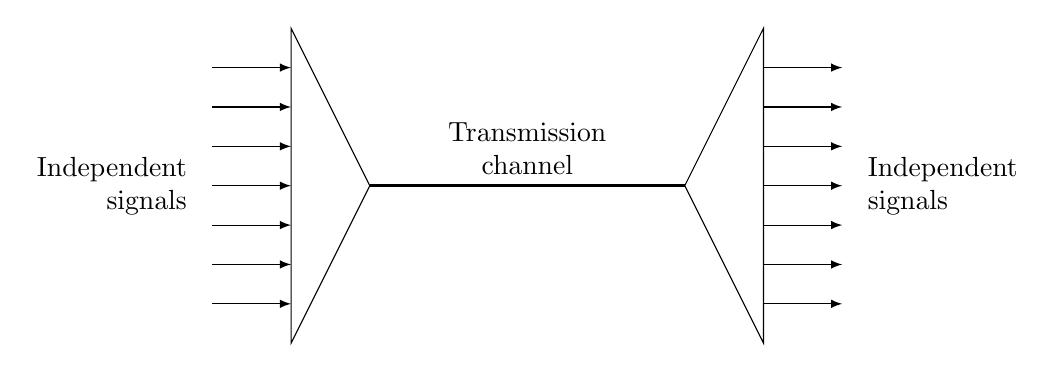
\begin{tikzpicture}
		\begin{scope}[shift={(-2,0)}]
			\draw (0,0) -- (-1,-2) -- (-1,2) -- cycle;
			\foreach \y in {1.5,1,0.5,0,-0.5,-1,-1.5}{
				\draw[-latex] (-2,\y) -- (-1,\y);
			}
			\node[anchor=east,align=right] at(-2.2,0) {Independent\\ signals};
		\end{scope}
		\begin{scope}[shift={(2,0)}]
			\draw (0,0) -- (1,-2) -- (1,2) -- cycle;
			\foreach \y in {1.5,1,0.5,0,-0.5,-1,-1.5}{
				\draw[-latex] (1,\y) -- (2,\y);
			}
			\node[anchor=west,align=left] at(2.2,0) {Independent\\ signals};
		\end{scope}
		\draw[very thick] (-2,0) -- node[midway,above,align=center]{Transmission\\ channel} (2,0);
	\end{tikzpicture}
	\caption[Principle of multiplexing]{Principle of multiplexing. Independent signals can be transmitted (quasi-) parallelly over the same transmission channel.}
\end{figure}

Multiple access methods are implemented in both the \emph{physical layer} (\acs{OSI} layer 1) and the \emph{data link layer} (\acs{OSI} layer 2).
\begin{itemize}
	\item The \index{medium access control} \textbf{\acf{MAC}} is a part of the \emph{data link layer} (\acs{OSI} layer 2). It contains the high-level logic which implements multiple access methods. It is responsible for the allocation of resources (scheduling). For example, it assigns \emph{spreading codes}, time-slots or sub-carriers to different users. The \ac{MAC} must provide reliable medium access. Data collisions of different users must be mitigated.
	\item The \emph{physical layer} (\acs{OSI} layer 1) changes the modulation and spreading parameters according to the instructions issued by the \emph{data link layer} (\acs{OSI} layer 2).
\end{itemize}

Reasons for multiple access:
\begin{itemize}
	\item \textbf{Number of users} -- A service is provided to lots of users.
	\item \textbf{Efficiency} -- Users occupy the medium for only a short time. Between the transmission bursts, other users can use the free medium.
	\item \textbf{Latency} -- Low latency can only be achieved if users can access the medium simultaneously.
\end{itemize}

\subsection{Space-Division Multiple Access}

A simple and \emph{non-spreading} method is \index{space-division multiple access} \textbf{\acf{SDMA}}.
\begin{itemize}
	\item Users are separated spatially.
	\item For wireless channels: The signals only have a limited range and cannot be received outside that range.
	\item For wired channels: The users are connected to different cables.
	\item The users are put into different spatial segments.
	\item All users can use the medium parallelly without interfering with each other.
\end{itemize}

\begin{figure}[H]
	\centering
	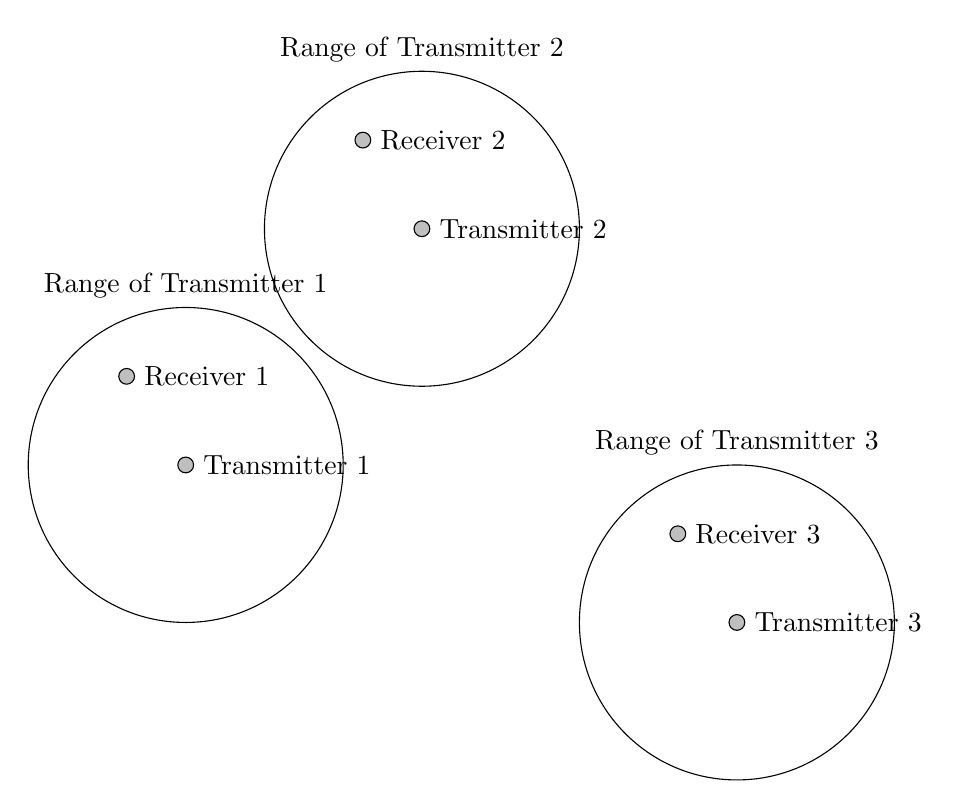
\begin{tikzpicture}
		\foreach \x/\y/\n in {0/0/1, 3/3/2, 7/-2/3}{
			\begin{scope}[shift={(\x,\y)}]
				\draw[fill=gray!50,draw=black] (0:0.1) arc(0:360:0.1) node[right,align=left]{Transmitter \n};
				\draw[draw=black] (90:2) arc(-270:90:2) node[above,align=center]{Range of Transmitter \n};
				\draw[fill=gray!50,draw=black] (120:1.3) arc(0:360:0.1) node[right,align=left]{Receiver \n};
			\end{scope}
		}
	\end{tikzpicture}
	\caption{Spatial separation as a method for reusing the frequency band}
\end{figure}

\subsection{Time-Division Multiple Access}

A \emph{multiple access} method derived from \ac{THSS} is \index{time-division multiple access} \textbf{\acf{TDMA}}.
\begin{itemize}
	\item Each user obtains one of the $M$ time-slot for exclusive usage.
	\item Usually, the time-slots are long enough so that a series of symbols can be transmitted for one user. In contrast to pure \ac{THSS}, where one symbol is transmitted as a chip, \ac{TDMA} transmits a series of symbols for user 1 and then hands over the transmission channel to the next user.
	\item \ac{ISI} between the users is an issue. Guard intervals must be inserted.
\end{itemize}

\begin{remark}
	Optionally, users can obtain multiple time-slot allocations to increase their data rate.
\end{remark}

\begin{figure}[H]
	\centering
	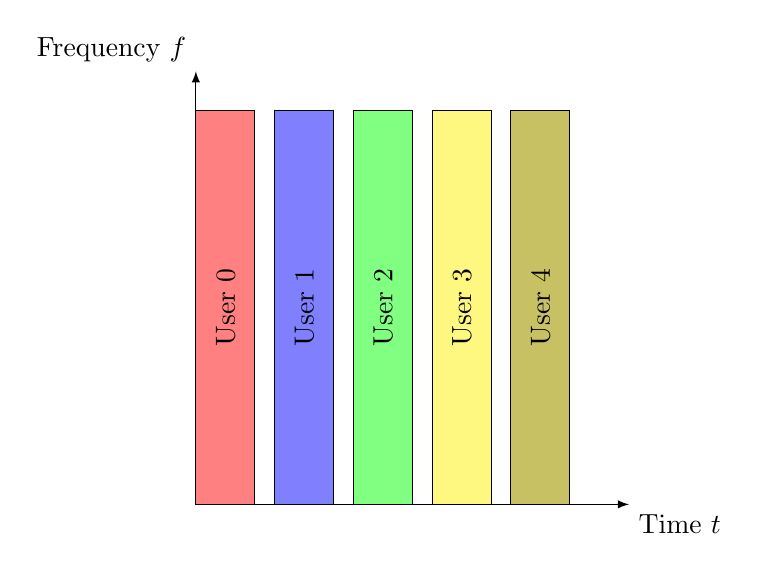
\begin{tikzpicture}[
		x={(0.5cm,0cm)},
		y={(0cm,0.5cm)},
	]
		\draw[-latex] (0,0) -- (11,0) node[below right,align=left]{Time $t$};
		\draw[-latex] (0,0) -- (0,11) node[above left,align=right]{Frequency $f$};
		
		\foreach \n/\c in {0/red, 1/blue, 2/green, 3/yellow, 4/olive}{
			\draw[fill=\c!50,draw=black] ({(\n*2)},0) -- ({(\n*2)},10) -- ({(\n*2)+1.5},10) -- ({(\n*2)+1.5},0) -- cycle;
			\node[align=center,rotate=90] at({(\n*2)+0.75},5) {User \n};
		}
	\end{tikzpicture}
	\caption[Time-slot allocation in a \acs{TDMA} system]{Time-slot allocation in a \acs{TDMA} system. In a \acs{TDMA} system, each user obtains a time-slot where it can exclusively use the whole bandwidth.}
\end{figure}

Advantages:
\begin{itemize}
	\item Only one carrier frequency $\rightarrow$ only one oscillator required for reception $\rightarrow$ simple receiver design
\end{itemize}

Drawbacks:
\begin{itemize}
	\item Time synchronization required
	\item Guard interval required
\end{itemize}

\subsection{Frequency-Division Multiple Access}

A \emph{multiple access} method derived from \ac{FHSS} is \index{frequency-division multiple access} \textbf{\acf{FDMA}}.
\begin{itemize}
	\item Each user obtains one of the $M$ sub-bands for exclusive usage.
	\item The \emph{spreading code} $C[m]$ is constant for each user and yields the sub-bands number.
	\item The frequency is not changed for a user. Thus, the frequency-hopping is replaced by a constant frequency.
	\item \emph{Inter-carrier interference} is an issue. Guard bands must be inserted.
\end{itemize}

\begin{remark}
	Optionally, users can obtain multiple sub-band allocations to increase their data rate.
\end{remark}

\begin{figure}[H]
	\centering
	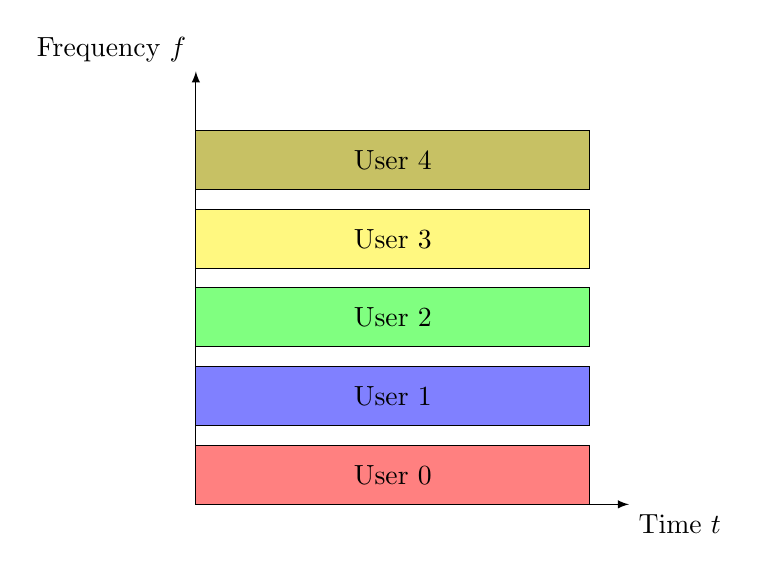
\begin{tikzpicture}[
		x={(0.5cm,0cm)},
		y={(0cm,0.5cm)},
	]
		\draw[-latex] (0,0) -- (11,0) node[below right,align=left]{Time $t$};
		\draw[-latex] (0,0) -- (0,11) node[above left,align=right]{Frequency $f$};
		
		\foreach \n/\c in {0/red, 1/blue, 2/green, 3/yellow, 4/olive}{
			\draw[fill=\c!50,draw=black] (0,{(\n*2)}) -- (10,{(\n*2)}) -- (10,{(\n*2)+1.5}) -- (0,{(\n*2)+1.5}) -- cycle;
			\node[align=center] at(5,{(\n*2)+0.75}) {User \n};
		}
	\end{tikzpicture}
	\caption[Sub-band allocation in an \acs{FDMA} system]{Sub-band allocation in an \acs{FDMA} system. In an \acs{FDMA} system, each user obtains a sub-band which it can exclusively use at any time.}
\end{figure}

Advantages:
\begin{itemize}
	\item No time synchronization required
\end{itemize}

Drawbacks:
\begin{itemize}
	\item More complex receiver design (many parallel oscillators or enhanced digital signal processing)
	\item Guard band required
\end{itemize}

\subsection{Hybrid TDMA and FDMA}

\ac{TDMA} and \ac{FDMA} can be combined to a hybrid system.
\begin{itemize}
	\item The allocation for both sub-bands and time-slots changes dynamically for each user.
	\item The pattern is determined by the \ac{MAC} layer (\acs{OSI} layer 2).
	\item Some users may lose allocations for the sake of enabling other users to use the transmission medium.
\end{itemize}

\begin{figure}[H]
	\centering
	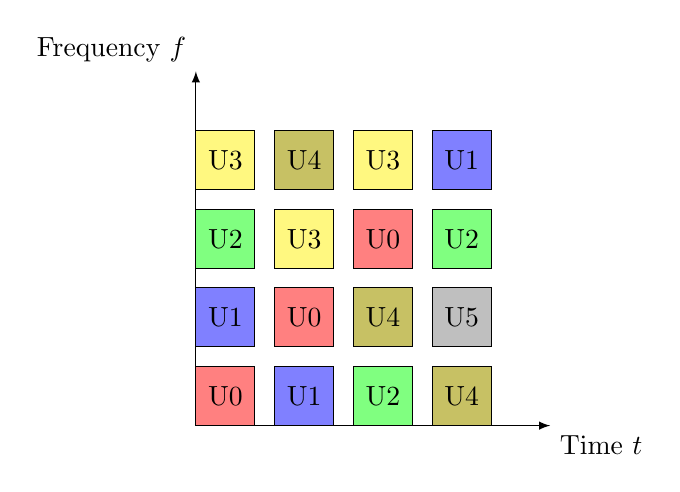
\begin{tikzpicture}[
		x={(0.5cm,0cm)},
		y={(0cm,0.5cm)},
	]
		\draw[-latex] (0,0) -- (9,0) node[below right,align=left]{Time $t$};
		\draw[-latex] (0,0) -- (0,9) node[above left,align=right]{Frequency $f$};
		
		\foreach \t/\f/\n/\c in {0/0/0/red, 0/1/1/blue, 0/2/2/green, 0/3/3/yellow,
			1/0/1/blue, 1/1/0/red, 1/2/3/yellow, 1/3/4/olive,
			2/0/2/green, 2/1/4/olive, 2/2/0/red, 2/3/3/yellow,
			3/0/4/olive, 3/1/5/gray, 3/2/2/green, 3/3/1/blue}{
			\draw[fill=\c!50,draw=black] ({(\t*2)},{(\f*2)}) -- ({(\t*2)+1.5},{(\f*2)}) -- ({(\t*2)+1.5},{(\f*2)+1.5}) -- ({(\t*2)},{(\f*2)+1.5}) -- cycle;
			\node[align=center] at({(\t*2)+0.75},{(\f*2)+0.75}) {U\n};
		}
	\end{tikzpicture}
	\caption{Sub-band and time-slot allocation in an \acs{TDMA}/\acs{FDMA} hybrid system}
\end{figure}

\begin{example}{2G cell phone -- \acs{GSM}}
	The 2G cell phone system (\acf{GSM}) uses a hybrid \acs{TDMA}/\acs{FDMA} scheme.
	\begin{itemize}
		\item 8 users can share a frequency.
		\begin{itemize}
			\item The \acs{TDMA} part uses 8 time-slots of $\SI{576.92}{\micro{}s}$ length.
			\item The 8 time-slots are arranged in a frame of $8 \cdot \SI{576.92}{\micro{}s} = \SI{4.615}{ms}$ length.
			\item Thus, a time-slot for each user repeats every $\SI{4.615}{ms}$.
			\item Frames are arranged in multi-frames, which themselves are arranged in super-frames, which themselves are arranged in hyper-frames.
			\item Each time-slot (if used for data traffic) can transport $\SI{114}{bit}$. (The frame has actually $\SI{156.25}{bit}$ used for data, synchronization, control information and guard interval.)
			\item The theoretical net data rate is $\SI{114}{bit} / \SI{4.615}{ms} = \SI{24.7}{kbit/s}$. This is sufficient to transmit voice.
			\item The real number of users is less than 8, because some time-slots are used for control information.
		\end{itemize}
		\item To enable, more than 8 users, a base station uses more than one frequency. Different users can be assigned different frequencies (\acs{FDMA}).
	\end{itemize}
\end{example}

\subsection{Code-Division Multiple Access}

All \emph{spread spectrum} technologies rely on \emph{spreading codes}.
\begin{itemize}
	\item The \emph{spreading codes} are the parameter of the \emph{spread spectrum} technology which defines how the signal power is spread.
	\item Using \index{orthogonal spreading codes} \textbf{orthogonal spreading codes}, multiple \emph{spread spectrum} signals can superimpose without interfering each other.
	\item Different \emph{orthogonal spreading codes} can be assigned to different users for \emph{multiple access}.
	\item The receiver is able to split the simultaneously transmitted signals of the different users using the \emph{orthogonal spreading codes}.
	\item Due to the code orthogonality, the users cannot interfere. The other user's signals will be noise to the receiver which is suppressed.
\end{itemize}

The \emph{multiple access} method using \emph{orthogonal spreading codes} is \index{code-division multiple access} \textbf{\acf{CDMA}}.

It can be subdivided according to the underlying \emph{spread spectrum} technology.
\begin{itemize}
	\item The \textbf{\acf{DS-CDMA}} uses \emph{\acf{DSSS}} with \emph{orthogonal spreading codes}.
	\item The \textbf{\acf{FH-CDMA}} uses \emph{\acf{FHSS}} with \emph{orthogonal spreading codes}.
	\item The \textbf{\acf{TH-CDMA}} uses \emph{\acf{THSS}} with \emph{orthogonal spreading codes}.
\end{itemize}

\subsubsection{Direct Sequence CDMA}

A \emph{\ac{CDMA} scheme} derived from \ac{DSSS} is \index{direct sequence code-division multiple access} \textbf{\acf{DS-CDMA}}.
\begin{itemize}
	\item \emph{Spreading codes} with a length of $L$ have $K$ combinations which are orthogonal.
	\item Each user obtains one of the $K$ \emph{orthogonal spreading codes} for exclusive usage.
	\item All users can transmit simultaneously using the whole bandwidth.
\end{itemize}

\begin{remark}
	Optionally, users can obtain multiple code allocations to increase their data rate.
\end{remark}

\begin{figure}[H]
	\centering
	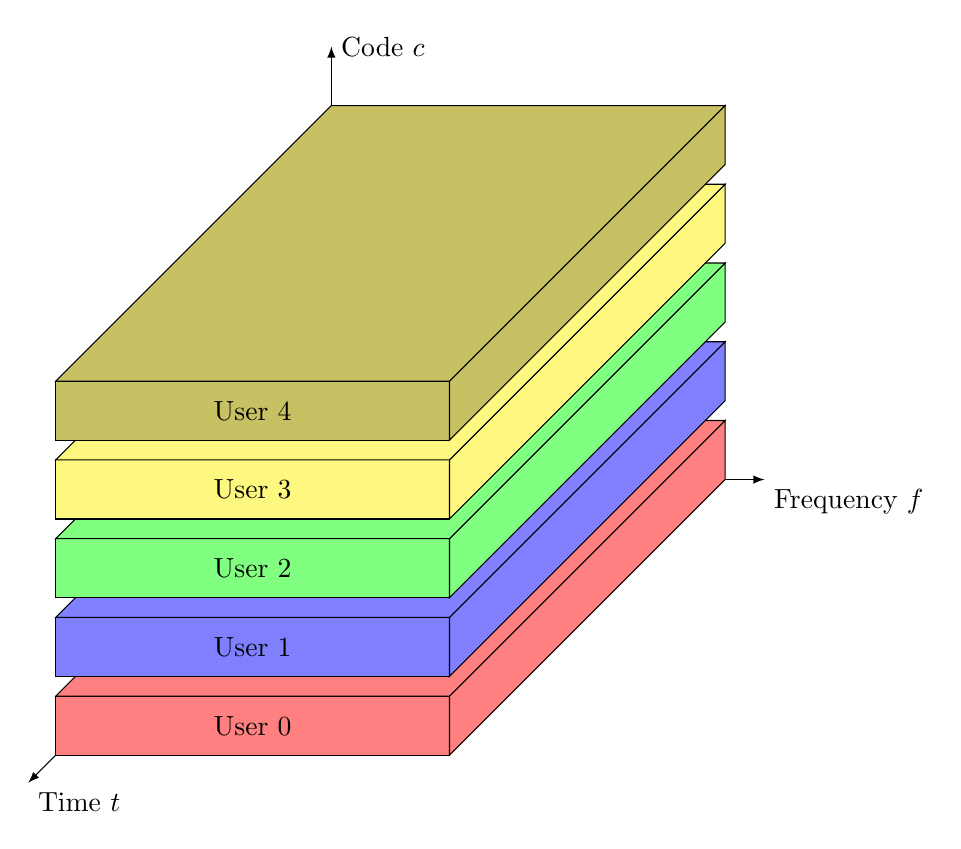
\begin{tikzpicture}[
		x={(-0.35cm,-0.35cm)},
		y={(0.5cm,0cm)},
		z={(0cm,0.5cm)},
	]
		\draw[-latex] (0,0,0) -- (11,0,0) node[below right,align=left]{Time $t$};
		\draw[-latex] (0,0,0) -- (0,11,0) node[below right,align=left]{Frequency $f$};
		\draw[-latex] (0,0,0) -- (0,0,11) node[right,align=left]{Code $c$};
		
		\foreach \n/\c in {0/red, 1/blue, 2/green, 3/yellow, 4/olive}{
			\draw[fill=\c!50,draw=black] (10,0,{(\n*2)}) -- (10,10,{(\n*2)}) -- (10,10,{(\n*2)+1.5}) -- (10,0,{(\n*2)+1.5}) -- cycle;
			\draw[fill=\c!50,draw=black] (10,10,{(\n*2)}) -- (0,10,{(\n*2)}) -- (0,10,{(\n*2)+1.5}) -- (10,10,{(\n*2)+1.5}) -- cycle;
			\draw[fill=\c!50,draw=black] (0,0,{(\n*2)+1.5}) -- (10,0,{(\n*2)+1.5}) -- (10,10,{(\n*2)+1.5}) -- (0,10,{(\n*2)+1.5}) -- cycle;
			\node[align=center] at(10,5,{(\n*2)+0.75}) {User \n};
		}
	\end{tikzpicture}
	\caption[Code allocation in a \acs{DS-CDMA} system]{Code allocation in a \acs{DS-CDMA} system. In a \acs{DS-CDMA} system, each user obtains a spreading code which is orthogonal to all other user's codes. The whole bandwidth is used by all users simultaneously.}
\end{figure}

Advantages:
\begin{itemize}
	\item Only one carrier $\rightarrow$ one analogue \ac{LO} $\rightarrow$ simple receiver design (analogue part)
	\item Bandwidth is used efficiently.
	\item Good noise immunity.
\end{itemize}

Drawbacks:
\begin{itemize}
	\item High requirements on digital signal processing (parallel detection of different codes)
	\item Transmitters must be able to adjust their transmission power. Transmitters which are closer to the receiver must reduce their power. Otherwise, the receiver would be over-driven due to the limited dynamic range. It then cannot receive far transmitters whose signals are relatively weak.
\end{itemize}

\subsubsection{Frequency-Hopping CDMA}

A \emph{\ac{CDMA} scheme} derived from \ac{FHSS} is \index{frequency-hopping code-division multiple access} \textbf{\acf{FH-CDMA}}.
\begin{itemize}
	\item In contrast to \ac{FDMA}, the frequency is not constant.
	\item The frequency is changed as defined by the \emph{orthogonal spreading codes}.
\end{itemize}

\begin{figure}[H]
	\centering
	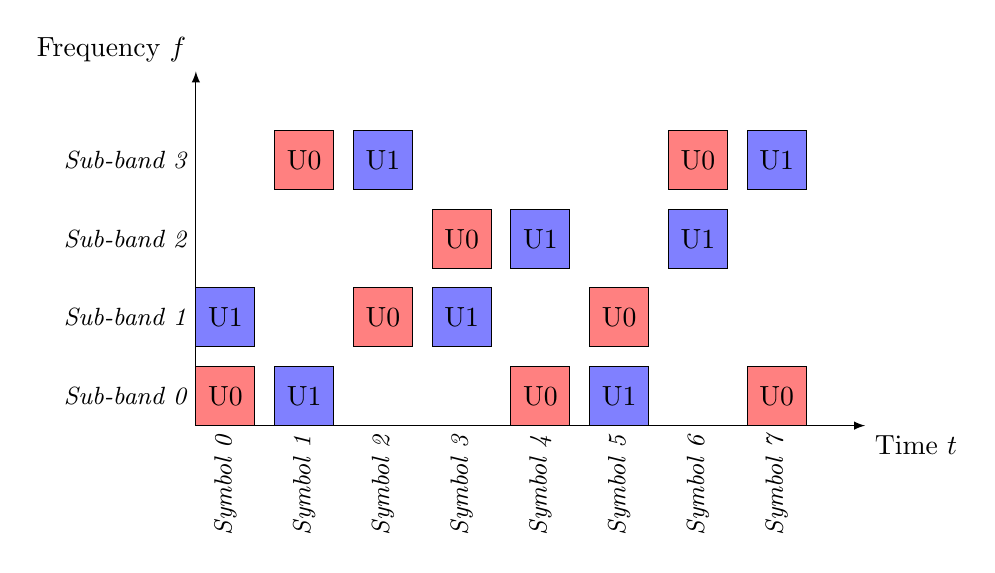
\begin{tikzpicture}[
		x={(0.5cm,0cm)},
		y={(0cm,0.5cm)},
	]
		\draw[-latex] (0,0) -- (17,0) node[below right,align=left]{Time $t$};
		\draw[-latex] (0,0) -- (0,9) node[above left,align=right]{Frequency $f$};
		
		\foreach \n in {0,1,2,3}{
			\node[anchor=east,align=right] at(0,{(\n*2)+0.75}) {\small \itshape Sub-band \n};
		}
		\foreach \n in {0,1,...,7}{
			\node[anchor=east,align=right,rotate=90] at({(\n*2)+0.75},0) {\small \itshape Symbol \n};
		}
		
		\foreach \t/\f/\n/\c in {0/0/0/red, 0/1/1/blue, 1/3/0/red, 1/0/1/blue, 2/1/0/red, 2/3/1/blue, 3/2/0/red, 3/1/1/blue, 4/0/0/red, 4/2/1/blue, 5/1/0/red, 5/0/1/blue, 6/3/0/red, 6/2/1/blue, 7/0/0/red, 7/3/1/blue}{
			\draw[fill=\c!50,draw=black] ({(\t*2)},{(\f*2)}) -- ({(\t*2)+1.5},{(\f*2)}) -- ({(\t*2)+1.5},{(\f*2)+1.5}) -- ({(\t*2)},{(\f*2)+1.5}) -- cycle;
			\node[align=center] at({(\t*2)+0.75},{(\f*2)+0.75}) {U\n};
		}
	\end{tikzpicture}
	\caption[Time-frequency distribution of symbols in an \acs{FH-CDMA} system]{Time-frequency distribution of symbols in an \acs{FH-CDMA} system. Due to the orthogonality of spreading codes, the symbols of different users in a \acs{FH-CDMA} system do not interfere. In this example the spreading factor is $M = 4$.}
\end{figure}

Benefits and drawbacks: See \ac{FDMA}

\subsubsection{Time-Hopping CDMA}

A \emph{\ac{CDMA} scheme} derived from \ac{THSS} is \index{time-hopping code-division multiple access} \textbf{\acf{TH-CDMA}}.
\begin{itemize}
	\item In contrast to \ac{TDMA}, the time-slot is not constant.
	\item The time-slot is changed as defined by the \emph{orthogonal spreading codes}.
\end{itemize}

\begin{figure}[H]
	\centering
	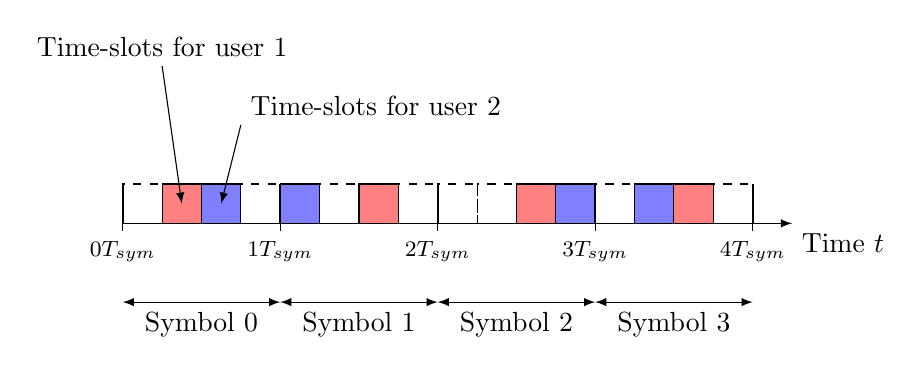
\begin{tikzpicture}[
		x={(0.5cm,0cm)},
		y={(0cm,0.5cm)},
	]
		\draw[-latex] (0,0) -- (17,0) node[below right,align=left]{Time $t$};
		
		\foreach \x/\c in {1/red, 2/blue, 4/blue, 6/red, 10/red, 11/blue, 13/blue, 14/red}{
			\draw[fill=\c!50,draw=black] ({(\x)},0) -- ({(\x)+1},0) -- ({(\x)+1},1) -- ({(\x)},1) -- cycle;
		}
		
		\foreach \x in {0,1,...,15}{
			\draw[dashed] ({(\x)},0) -- ({(\x)+1},0) -- ({(\x)+1},1) -- ({(\x)},1) -- cycle;
		}
		\foreach \n in {0,1,2,3,4}{
			\draw ({\n*4},0) -- ({\n*4},-0.2) node[below,align=center]{\footnotesize $\n T_{sym}$};
			\draw[thick] ({\n*4},0) -- ({\n*4},1);
		}
	
		\foreach \n in {0,1,2,3}{
			\draw[latex-latex] ({\n*4},-2) --  node[midway,below,align=center]{Symbol \n} ({(\n+1)*4},-2);
		}
	
		\draw[latex-] (1.5,0.5) -- (1,4) node[above,align=center]{Time-slots for user 1};
		\draw[latex-] (2.5,0.5) -- (3,2.5) node[above right,align=left]{Time-slots for user 2};
	\end{tikzpicture}
	\caption[Symbol distribution of different users in a \acs{TH-CDMA} system]{Symbol distribution of different users in a \acs{TH-CDMA} system. In this example the spreading factor is $M = 4$.}
\end{figure}

Benefits and drawbacks: See \ac{TDMA}

\subsection{Orthogonal Frequency-Division Multiple Access}

The \index{orthogonal frequency-division multiple access} \textbf{\acf{OFDMA}} is an extension of the \ac{FDMA} using \emph{orthogonal sub-carrier}. The \ac{OFDMA} method is implemented by a \ac{OFDM} system.
\begin{itemize}
	\item The sub-band allocation equals that of \ac{FDMA}.
	\item The carriers of the sub-bands are orthogonal. Guard bands are not required. The different users will not interfere.
\end{itemize}


\section{CDMA Codes}

\emph{Spreading codes} must have special properties to enable \emph{multiple access}.
\begin{itemize}
	\item The \index{autocorrelation function} \textbf{cross-correlation function} of \emph{spreading codes} shall have two values.
	\begin{itemize}
		\item A peak at time $0$. That is, the code can detect itself.
		\item Close to zero every other times. The code should not detect time-delayed replica of itself.
	\end{itemize}
	\item The \index{cross-correlation function} \textbf{cross-correlation function} of \emph{spreading codes} to other codes shall be close to zero. Signals spread with different codes shall be suppressed as good as possible.
\end{itemize}

Let's consider \acs{DS-CDMA}, which implements the symbol spreading by multiplying each symbol with the \emph{spreading code} and thereby increasing the \emph{chip rate}. At the receiver side, there are two cases.
\begin{itemize}
	\item \textbf{Synchronous} -- The signals of all received users are synchronized. All symbols start at the same time and have the same period.
	\item \textbf{Asynchronous} -- The signals of all received users are \underline{not} synchronized. There can be a random time-shift, i.e, phase-shift, of the symbols of different users.
\end{itemize}

\subsection{Synchronous \acs{DS-CDMA}}

For the synchronous case, it is sufficient if the \emph{spreading codes} are \emph{orthogonal}.

Two codes of length $L$ $\vect{C}_{L,1}$ and $\vect{C}_{L,2}$ are \index{orthogonal codes} \textbf{orthogonal codes} if their inner product is zero.
\begin{equation}
	0 \stackrel{!}{=} \left\langle \vect{C}_{L,1}, \vect{C}_{L,2} \right\rangle = \sum\limits_{l = 0}^{L-1} \vect{C}_{L,1}[l] \cdot \vect{C}_{L,2}[l]
\end{equation}

One set of codes, which is orthogonal, are \index{Welsh codes} \textbf{Welsh codes}. They are created out of \textbf{Hadamard matrices}.

\begin{definition}{Hadamard matrices}
	\index{Hadamard matrix} \textbf{Hadamard matrices} is a $L \times L$ matrix. Where $L = 2^k$ (with $k \in \mathbb{N}$) is a power of two.
	
	A Hadamard matrix $\mat{H}_{2L}$ of the order $2L$ is constructed from Hadamard matrices $\mat{H}_{L}$ of the order $L$.
	\begin{equation}
		\mat{H}_{2L} = \left[\begin{matrix}
			\mat{H}_{L} & \mat{H}_{L} \\
			\mat{H}_{L} & -\mat{H}_{L} \\
		\end{matrix}\right]
	\end{equation}
	
	Examples:
	\begin{equation}
		\mat{H}_{1} = \left[\begin{matrix} 1 \\ \end{matrix}\right]
	\end{equation}
	\begin{equation}
		\mat{H}_{2} = \left[\begin{matrix}
			1 & 1 \\
			1 & -1 \\
		\end{matrix}\right]
	\end{equation}
	\begin{equation}
		\mat{H}_{4} = \left[\begin{matrix}
			1 & 1 & 1 & 1 \\
			1 & -1 & 1 & -1 \\
			1 & 1 & -1 & -1 \\
			1 & -1 & -1 & 1 \\
		\end{matrix}\right]
	\end{equation}
\end{definition}

The rows or columns, respectively, of Hadamard matrices are orthogonal to each other. They can be directly used as spreading codes. The order $L$ of the Hadamard matrix defines the code length.

Furthermore, the $L$ codes are not only orthogonal to each other.
\begin{itemize}
	\item Imagine that you have a Welsh code $\vect{C}_{L,1} = \left[1, 1, -1, -1\right]$ with $L_1 = 4$.
	\item In addition, you have a Welsh code $\vect{C}_{L,2} = \left[1, -1\right]$ with $L_2 = \frac{1}{2} L_1 = 2$.
	\item \textbf{Both codes are orthogonal, despite their different length.}
	\item $\vect{C}_{L,2}$ can be periodically continued to $\left[1, -1, 1, -1\right]$, which is orthogonal to $\vect{C}_{L,1}$.
	\item The chip rate of both codes must be equal. \begin{remark}Remember that we are in the synchronous case here.\end{remark}
\end{itemize}

What is the use of this property?
\begin{itemize}
	\item $\vect{C}_{L,2}$ requires less chips for encoding one data symbol than $\vect{C}_{L,1}$ ($2$ versus $4$).
	\item $\vect{C}_{L,2}$ has the double data rate than $\vect{C}_{L,1}$, whilst the chip rate remains constant.
	\item \textbf{It is possible to have different data streams with different data rates in the same transmission channel.}
	\item The \emph{spreading factor}, which is responsible for the data rate, can be adapted.
	\item The Welsh code is an \index{orthogonal variable spreading factor} \textbf{\acf{OVSF}} code.
\end{itemize}

However, not each $L_1$ code is orthogonal to any $L_2$ code. The relation of orthogonality of codes with different length can be depicted in the \acs{OVSF} code tree (Figure \ref{fig:ch07:ovsf_code_tree}).
\begin{figure}[H]
	\centering
	\begin{tikzpicture}
		\draw (-0.5,0) -- node[midway,above,align=center]{$\vect{C}_{1,1} = \left[1\right]$} (2,0);
		\draw (2,4) -- (2,-4);
		
		\foreach \y/\n/\v in {4/1/{1,1}, -4/2/{1,-1}}{
			\draw (2,\y) -- node[midway,above,align=center]{$\vect{C}_{2,\n} = \left[\v\right]$} (5,\y);
			\draw (5,{\y+2}) -- (5,{\y-2});
		}
	
		\foreach \y/\n/\v in {6/1/{1,1,1,1}, 2/2/{1,1,-1,-1}, -2/3/{1,-1,1,-1}, -6/4/{1,-1,-1,1}}{
			\draw (5,\y) -- node[midway,above,align=center]{$\vect{C}_{4,\n} = \left[\v\right]$} (9,\y);
			\draw (9,{\y+1}) -- (9,{\y-1});
		}
	
		\foreach \y/\n/\v in {7/1/{1,1,1,1,1,1,1,1}, 5/2/{1,1,1,1,-1,-1,-1,-1}, 3/3/{1,1,-1,-1,1,1,-1,-1}, 1/4/{1,1,-1,-1,-1,-1,1,1}, -1/5/{1,-1,1,-1,1,-1,1,-1}, -3/6/{1,-1,1,-1,-1,1,-1,1}, -5/7/{1,-1,-1,1,1,-1,-1,1}, -7/8/{1,-1,-1,1,-1,1,1,-1}}{
			\draw (9,\y) -- node[midway,above,align=center]{$\vect{C}_{8,\n} = \left[\v\right]$} (16,\y);
		}
	
		\foreach \x/\s in {1.8/1, 4.8/2, 8.8/4, 15.8/8}{
			\draw[dotted] (\x,9) -- (\x,-7);
		}
		\foreach \x/\s in {0.75/1, 3.5/2, 7/4, 12.5/8}{
			\node[anchor=south,align=center] at(\x,8) {\small Spreading\\ factor \s};
		}
	\end{tikzpicture}
	\caption[\acs{OVSF} code tree]{\acs{OVSF} code tree. Codes of different length \underline{are orthogonal} if they \underline{do not reside} in same branch of the tree. Codes \underline{are not} orthogonal if the shorter code \underline{can be found} inside of the longer code.}
	\label{fig:ch07:ovsf_code_tree}
\end{figure}

The rules for creating the \acs{OVSF} code tree are (derived from the construction rules of the Hadamard matrix):
\begin{itemize}
	\item The parent node in the tree is $\vect{C}_{n,k}$ ($n$ is the code length, $k$ is the index).
	\item The child nodes are:
	\begin{itemize}
		\item $\vect{C}_{2n,2k-1} = \left[\vect{C}_{n,k}, \vect{C}_{n,k}\right]$
		\item $\vect{C}_{2n,2k} = \left[\vect{C}_{n,k}, -\vect{C}_{n,k}\right]$
	\end{itemize}
\end{itemize}

\subsection{Asynchronous \acs{DS-CDMA}}

Welsh code have excellent cross-correlation properties. But, Welsh codes \underline{do not} have good autocorrelation properties.
\begin{itemize}
	\item The \emph{autocorrelation function} of Welsh codes might show more than one peak.
	\item Therefore, Welsh codes \underline{are not} suitable for asynchronous \ac{DS-CDMA}, where symbols of different users may be received with a time-shift.
	\item The correlator in the receiver will not be able to synchronize to the time-shift.
\end{itemize}

For asynchronous \ac{DS-CDMA}, codes must have good autocorrelation properties.
\begin{itemize}
	\item They shall only have one peak, so that the correlator in the receiver can determine the time-shift and synchronize itself.
	\item The cross-correlation to other codes shall be close to uero.
	\item Good codes are \index{pseudo-random number code} \textbf{\acf{PRN} codes}.
	\begin{itemize}
		\item There are equal numbers of $+1$'s and $-1$'s in the code sequence.
		\item The $+1$'s and $-1$'s are equally distributed.
	\end{itemize}
	\item The codes are not necessarily orthogonal. Only the autocorrelation and cross-correlation properties are important.
\end{itemize}

Examples of such codes (without going into detail):
\begin{itemize}
	\item Gold codes
	\item Kasami codes
\end{itemize}

%\begin{example}{3G cell phone -- \acs{UMTS}}
%\end{example}

\section{Duplexing}

Usually, there is not only one dedicate transmitter and one dedicate receiver (simplex). The terminals in a digital communication system may both transmit and receive (duplex). Example: A cell phone must be able to transmit and receive data, because the voice channel is bi-directional.

The communication relations (between two terminals) can be classified:
\begin{itemize}
	\item \textbf{Simplex} -- One only device is transmitting. The other one is only receiving.
	\item \textbf{Half-duplex} -- Both terminals transmit and receive. Only one of the two devices can transmit at once. The devices exchange their transmitter and receiver roles, when one device finished its transmission and the other one wants to transmit.
	\item \textbf{Full-duplex} -- Both terminals transmit and receive simultaneously.
\end{itemize}

Examples:
\begin{itemize}
	\item Simplex: Radio broadcasting, television broadcasting
	\item Half-duplex: Walkie-talkie (push-to-talk button to switch from reception to transmission)
	\item Full-duplex: telephone, cellphone (both persons can speak simultaneously)
\end{itemize}

Simplex and half-duplex can be easily implemented using the same transmission medium. It must only be ensured that only one device transmits at once.

Full-duplex is more challenging, because both devices want to both transmit and receive simultaneously.

\subsection{Frequency-Division Duplex}

The \index{frequency-division duplex} \textbf{\acf{FDD}} uses two frequencies.
\begin{itemize}
	\item Frequency $f_1$ is used by device 1 for transmission and by device 2 for reception.
	\item Frequency $f_2$ is used by device 2 for transmission and by device 1 for reception.
\end{itemize}
The transmission is perfectly simultaneous.

\ac{FDD} is the \emph{duplexing method} derived from \ac{FDMA}.

\begin{remark}
	Like in an \ac{FDMA} system, guard bands must be inserted to mitigate inter-carrier interference.
\end{remark}

Examples:
\begin{itemize}
	\item 2G cell phone (\acs{GSM}) according to the \acs{ETSI} TS 145 002 Standard \cite{etsits145002}
\end{itemize}

\subsection{Time-Division Duplex}

The \index{time-division duplex} \textbf{\acf{TDD}} uses two sequential time-slots in the same frequency band.
\begin{itemize}
	\item Time-slot 1 is used by device 1 for transmission and by device 2 for reception.
	\item Time-slot 2 is used by device 2 for transmission and by device 1 for reception.
	\item Afterwards, time-slot 1 starts again.
\end{itemize}
In fact, this is a half-duplex method. But, the time-slots are so short that the user will not notice the switching between the time-slots. The duplexing is \emph{quasi-full-duplex}.

\ac{TDD} is the \emph{duplexing method} derived from \ac{TDMA}.

\begin{remark}
	Like in an \ac{TDMA} system, guard intervals must be inserted to mitigate \ac{ISI}.
\end{remark}

Examples:
\begin{itemize}
	\item \acf{TETRA}: trunked radio system for professional mobile radio according to the \acs{ETSI} EN 300 392 Standard \cite{en300392}
\end{itemize}

\begin{figure}[H]
	\centering
	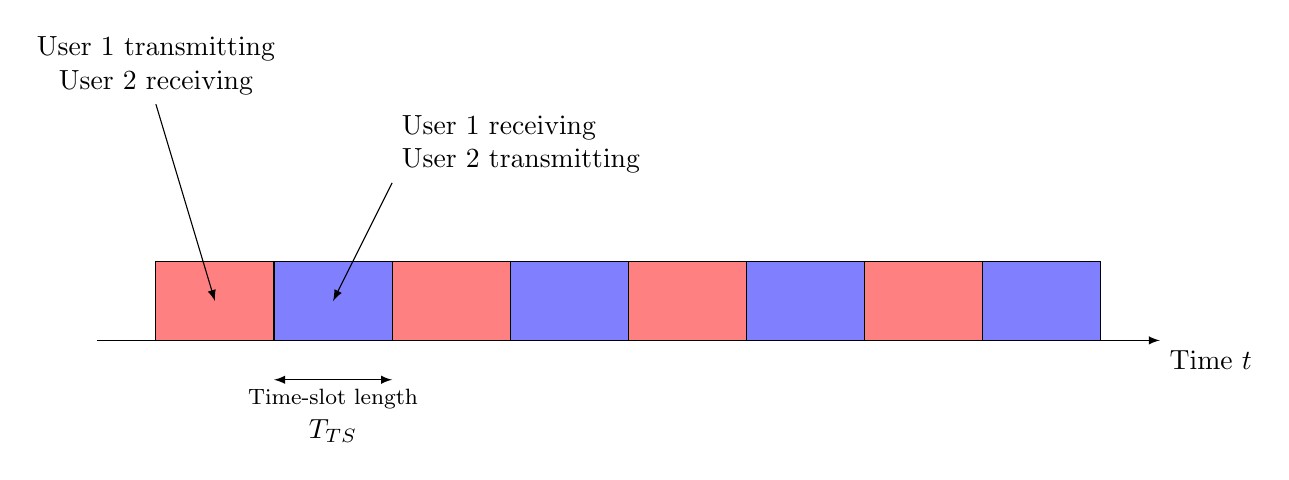
\begin{tikzpicture}[
		x={(1.5cm,0cm)},
		y={(0cm,1cm)},
	]
		\draw[-latex] (-0.5,0) -- (8.5,0) node[below right,align=left]{Time $t$};
		
		\foreach \x in {0,2,4,6}{
			\draw[fill=red!50,draw=black] ({(\x)},0) -- ({(\x)+1},0) -- ({(\x)+1},1) -- ({(\x)},1) -- cycle;
			%\node[align=center] at({(\x)+0.5},0.5) {User 1 Tx\\ User 2 Rx};
		}
		\draw[latex-] (0.5,0.5) -- (0,3) node[above,align=center]{User 1 transmitting\\ User 2 receiving};
	
		\foreach \x in {1,3,5,7}{
			\draw[fill=blue!50,draw=black] ({(\x)},0) -- ({(\x)+1},0) -- ({(\x)+1},1) -- ({(\x)},1) -- cycle;
			%\node[align=center] at({(\x)+0.5},0.5) {User 1 Rx\\ User 2 Tx};
		}
		\draw[latex-] (1.5,0.5) -- (2,2) node[above right,align=left]{User 1 receiving\\ User 2 transmitting};
	
		\draw[latex-latex] (1,-0.5) -- node[midway,below,align=center]{\footnotesize Time-slot length\\ $T_{TS}$} (2,-0.5);
	\end{tikzpicture}
	\caption{Distribution of transmission and reception time-slots (without guard intervals) in a \acs{TDD} system}
\end{figure}


\nocite{ipatov2005}

\phantomsection
\addcontentsline{toc}{section}{References}
\printbibliography[heading=subbibliography]
\end{refsection}

